In this chapter, the \textit{SLDC} framework is applied to the problem presented in Chapter \ref{chap:context} : the nodule malignancy assessment. This problem is effectively an instance of the object detection and classification problem. Indeed, the goal is to diagnose malignancy by the presence or absence of cells or groups of cells having particular characteristics in digitized microscope slides. This problem is a good use case for the \textit{SLDC} framework: the images are large (i.e. typically 15 giga-pixels), two distinct categories of objects must be found (namely cells and groups of cells) and some of these objects can be included into others which can be handled using dispatching and chaining.  

An introduction to the thyroid problem as well as the underlying implementation challenges are presented in Section \ref{sec:thyroid_impl_issue}. Then, the workflow developed in \cite{adeblire2013} is briefly presented and its performances are assessed in Section \ref{sec:thyroid_adeblire_algo}. Especially, some flawed steps are highlighted and some improvements are proposed. Then, the implementation of the improved workfow is detailed in Section \ref{sec:thyroid_implementation}. Finally, the performances of this implementation are analyzed in Section \ref{sec:thyroid_perf}.

\section{Problem and underlying challenges}
\label{sec:thyroid_impl_issue}
The problem consists in finding cells with inclusion and proliferative architectural patterns in large digitized microscope slides. To perform this detection, a dataset containing approximately 6000 annotations was created by experts on the Cytomine platform (see Section \ref{}). The major challenges involved with this problem are detailed hereafter. 

\paragraph{Image quality} While the image resolution is more than acceptable, the images themselves are by nature not very well suited for object extraction. Indeed, the objects of interests are surrounded with a lot of other undesirable objects. Moreover, due to the imprecise nature of the staining performed before digitization, some staining variations can appear across slides or within a slide. 

\paragraph{Image size} As explained in Section \ref{sssec:detection_thyroid_dataset}, image sizes range from 4 giga-pixels to 18 giga-pixels. Therefore, the various processing steps should be as efficient as possible to avoid huge execution times. Also, accessing the images must be done through HTTP requests. Therefore, a particular attention should be paid to the number of requests to be executed for fetching the image. Especially, some caching policy might be needed to reduce those requests execution time overhead. 

\paragraph{Class imbalance} The dataset of annotations is relatively balanced if all terms are considered separately. However, grouping terms for expressing the detection as a binary (or ternary) problem results in class imbalance, especially for the cells with inclusion versus normal cells problem. 

\paragraph{Human annotations} The human annotations are imperfect as experts usually annotate objects roughly (i.e. an annotation can be larger than the actual object). Moreover, some annotation drawing tools provided on the Cytomine platform generate particular shapes such as circles or rectangles. Assuming that an algorithm will annotate the cells more precisely, the resulting  differences in terms of geometry and information content of the crops might affect the performances of any classifier fitted on those experts' annotations. 

\section{First workflow}
\label{sec:thyroid_adeblire_algo}

The workflow developed by Antoine Deblire in \cite{adeblire2013} is summarized in Figure \ref{fig:workflow_adeblire}. The idea behind this workflow is fairly simple. First, a segmentation is applied to the whole slide to extract standalone cells and architectural patterns (step 4.3). The detected objects are then differentiated using their area and circularity (step 4.4) and dispatched to a classifier (steps 4.6). Especially, architectural patterns are classified as proliferative or non-proliferative by a first classifier and the cells are classified as inclusion or normal by a second one. Then, architectural patterns are segmented using a second segmentation algorithm (step 4.5) to extract the cells they contain and thos cells are also passed to the cell classifier. The next sections aim at explaining more thoroughly those steps.

\begin{figure}
	\center
	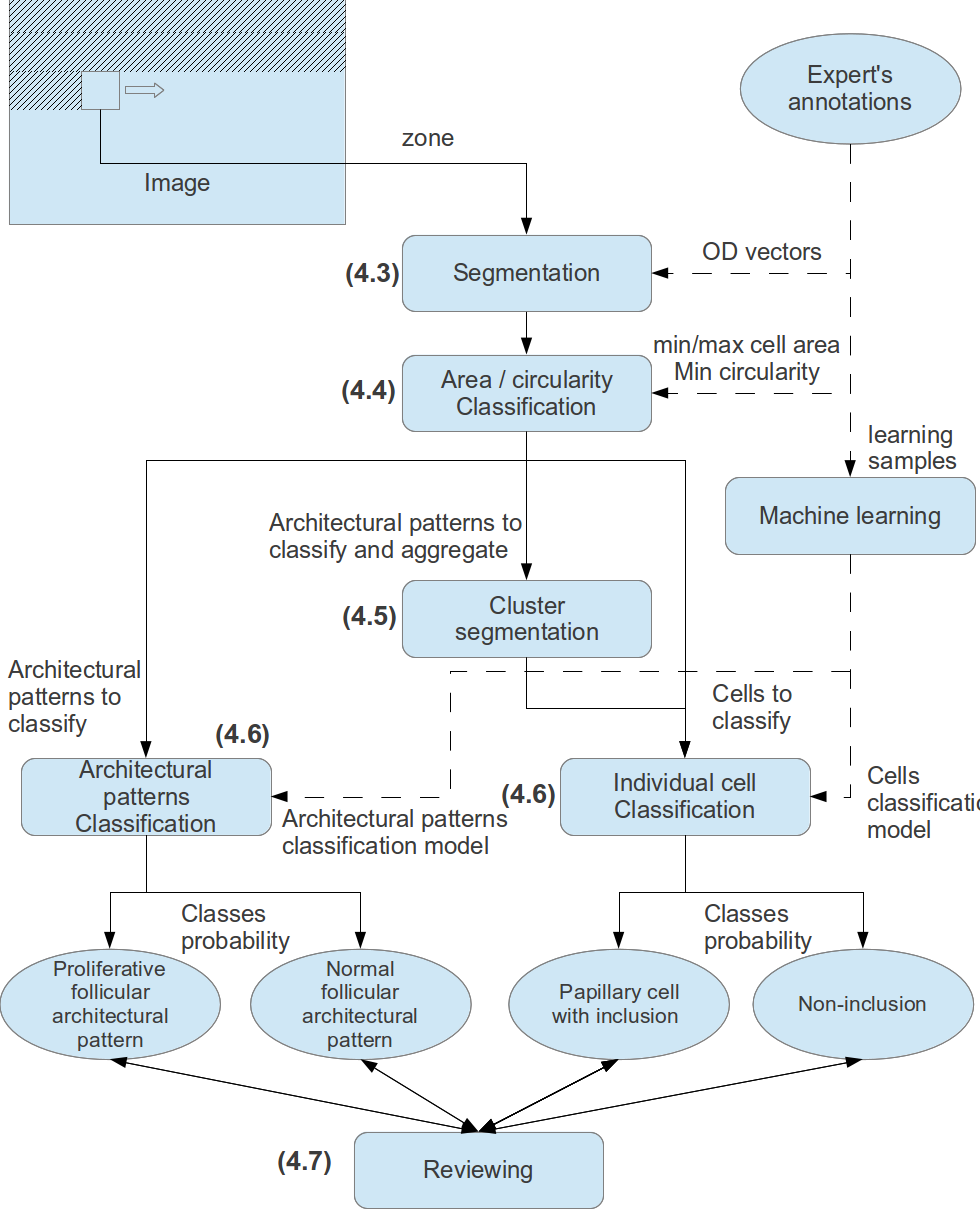
\includegraphics[scale=0.95]{image/adeblire_workflow.png}
	\caption{Antoine Deblire's workflow (source: \cite{adeblire2013})}
	\label{fig:workflow_adeblire}
\end{figure}

\subsection{Segmentation procedures}
\label{ssec:segmentation_proc}
Segmentation is carried out in two steps. The first segmentation procedure was designed for processing the whole slide and relies on a process called color deconvolution \cite{ruifrok2001quantification}. This process consists in retrieving the stains concentration of the objects contained in the image based on the RGB values of the pixels (see Section \ref{} for the staining process applied to the slides before digitization). Especially, given that the original slide was prepared with $S$ stains, the color deconvolution process generates a set of $S$ images where the pixel $p^s_{ij}$ of an image is the concentration level of the stain $s$ in the pixel $p^o_{ij}$ of the original image. This process is particularly useful in this case because cells and patterns have a high concentration of a given stain. The first segmentation procedure starts by generating the concentration image for the first stain. As pixels with a high concentration are supposed to be in an object of interest, a first binary mask is created by thresholding the concentration image. Three morphological operations are then successively applied to the segmentation mask:

\begin{itemize}
	\item Morphological closing to eliminate small holes in the detected objects.
	\item Morphological opening to eliminate small objects supposed to be irrelevant due to their size.
	\item Morphological closing to unify close neighbouring objects supposed to be part of a pattern.
\end{itemize}

Some example segmentations are provided in Figure \ref{fig:first_seg_example_high_stain} and \ref{fig:first_seg_examples}. It seems that the procedure is able to detect most of the objects of interest although it sometimes fails at covering those objects' whole area. For instance, in the fourth example image, there is a hole in the mask inside the pattern and this hole covers some cells that should be included in the mask. On the fifth example, one can see three standalone objects above the central pattern. Those objects' masks are smaller than their corresponding cells. Also, on some images, regions containing a high stain concentration were marked as object by the segmentation. This can be seen on the first example image in Figure \ref{fig:first_seg_example_high_stain} where a portion of the slide background was detected as pattern. 

\begin{figure}
	\center	
	\subfigure{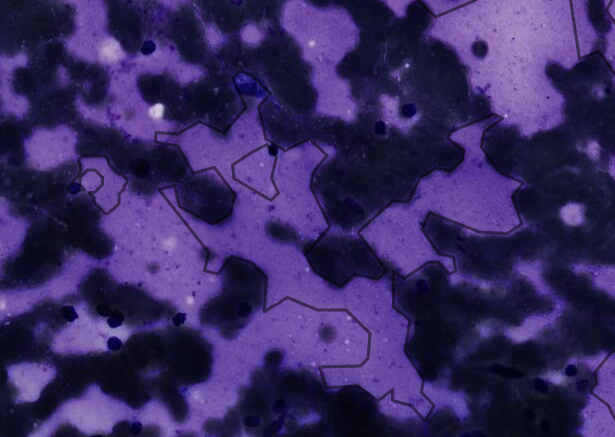
\includegraphics[scale=0.35]{image/seg_fail_stain_nomask.png}}
	\subfigure{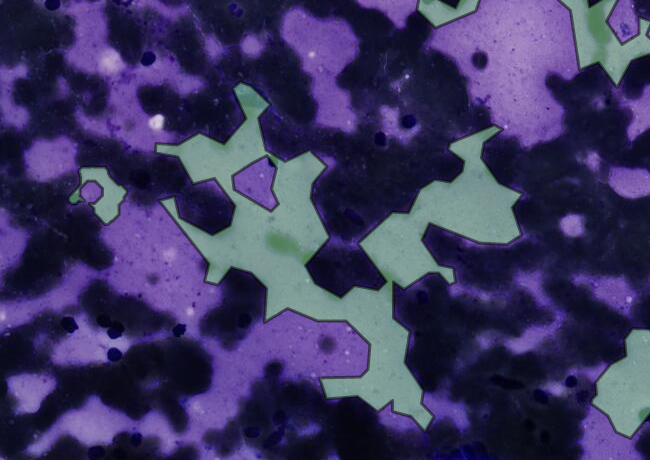
\includegraphics[scale=0.33]{image/seg_fail_stain_mask.png}}
	\caption{Background detected by the segmentation as an object. The background was segmented because of a higher stain concentration which is visible on the left image. The segmented area is delimited by the annotation on the right image.}
	\label{fig:first_seg_example_high_stain}
\end{figure}
\begin{figure}
	\center
	\subfigure{
		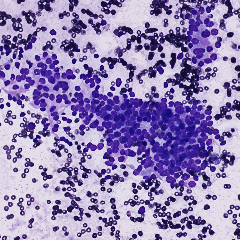
\includegraphics[scale=0.5]{image/slide_segmentation_0_in.png}
		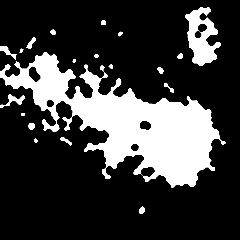
\includegraphics[scale=0.5]{image/slide_segmentation_0_out.png}
		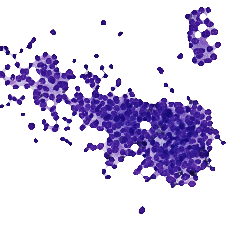
\includegraphics[scale=0.5]{image/slide_segmentation_0_masked.png}
	} \\
	\subfigure{
		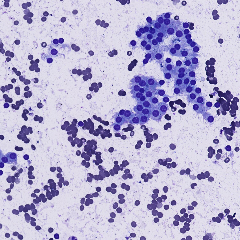
\includegraphics[scale=0.5]{image/slide_segmentation_1_in.png}
		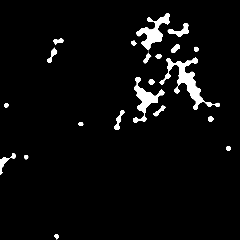
\includegraphics[scale=0.5]{image/slide_segmentation_1_out.png}
		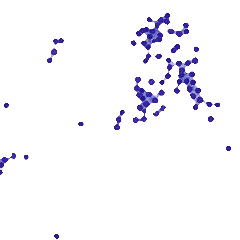
\includegraphics[scale=0.5]{image/slide_segmentation_1_masked.png}
	} \\
	\subfigure{
		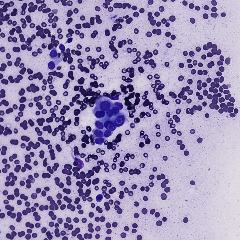
\includegraphics[scale=0.5]{image/slide_segmentation_2_in.png}
		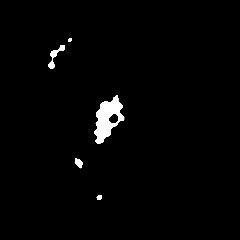
\includegraphics[scale=0.5]{image/slide_segmentation_2_out.png}
		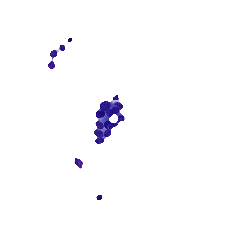
\includegraphics[scale=0.5]{image/slide_segmentation_2_masked.png}
	} \\
	\subfigure{
		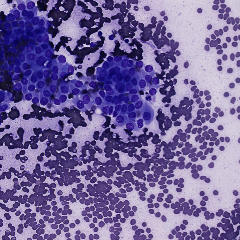
\includegraphics[scale=0.5]{image/slide_segmentation_3_in.png}
		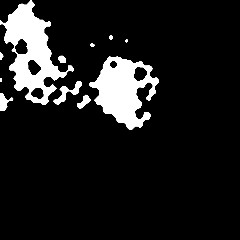
\includegraphics[scale=0.5]{image/slide_segmentation_3_out.png}
		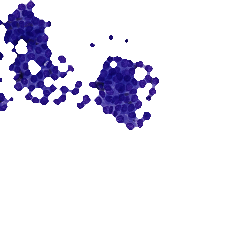
\includegraphics[scale=0.5]{image/slide_segmentation_3_masked.png}
	}
	\caption{Examples of slide segmentation. For each example, three images are given: the original image to the left, the segmentation mask in the center and to the right, the original image in which the pixels that do not belong to the segmentation mask were replaced by white pixels.}
	\label{fig:first_seg_examples}
\end{figure}

The second segmentation procedure is applied to the detected patterns and was designed to isolate individual cells inside those patterns. The implementation is slightly more complicated than the first (see \cite{adeblire2013} for the full procedure). Similarly, it starts with a color deconvolution to highlight the cells. However, the stain concentration image is not transformed into a binary mask using a fixed threshold but using Otsu's method \cite{otsu1975threshold}. Using the \texttt{findContour} procedure of the OpenCV library as well as morphological operations, independent cells are located and cleaned one after another. Finally, a watershed algorithm is applied to separate cells that overlap. Some example segmentations are provided in Figure \ref{fig:second_seg_examples}. The segmentation seems to work relatively well on "clean" patterns: that is, where cells do not overlap much and are clearly distinguishable from the pattern background (see the first two examples in Figure \ref{fig:second_seg_examples}). On "dirty" patterns however, the segmentation performs poorly as it either returns large patches which do not correspond to cells or fails to separate overlapping cells (see the two last examples in Figure \ref{fig:second_seg_examples}). In both cases, one can notice that the detected cells are slightly under-segmented (i.e. the segmentation mask is smaller than the actual object).

\begin{figure}
	\center
	\subfigure{
		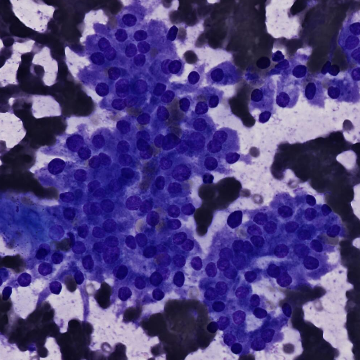
\includegraphics[scale=0.33]{image/aggr_segment_12_in.png}
		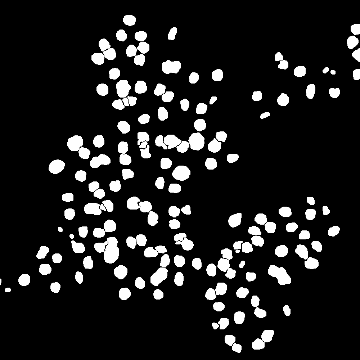
\includegraphics[scale=0.33]{image/aggr_segment_12_out.png}
		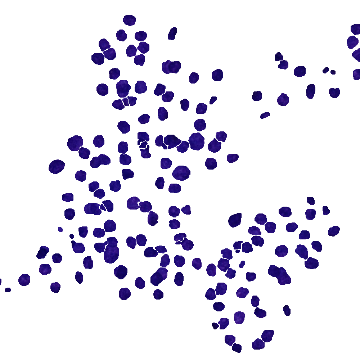
\includegraphics[scale=0.33]{image/aggr_segment_12_masked.png}
	} \\
	\subfigure{
		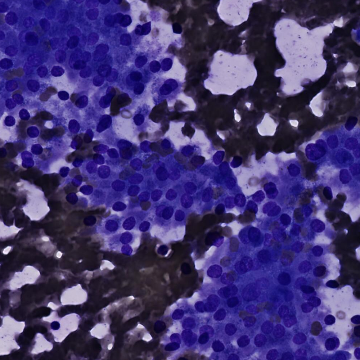
\includegraphics[scale=0.33]{image/aggr_segment_2_in.png}
		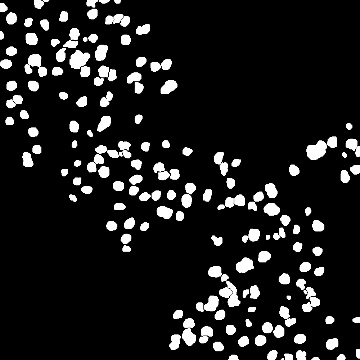
\includegraphics[scale=0.33]{image/aggr_segment_2_out.png}
		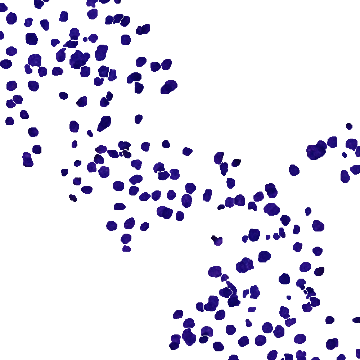
\includegraphics[scale=0.33]{image/aggr_segment_2_masked.png}
	} \\
	\subfigure{
		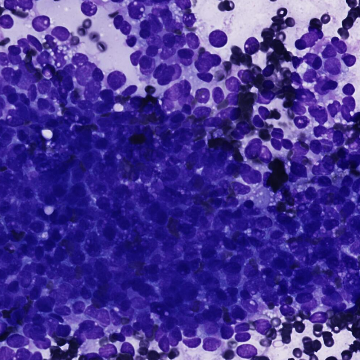
\includegraphics[scale=0.33]{image/aggr_segment_5_in.png}
		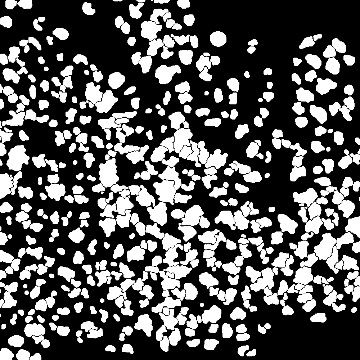
\includegraphics[scale=0.33]{image/aggr_segment_5_out.png}
		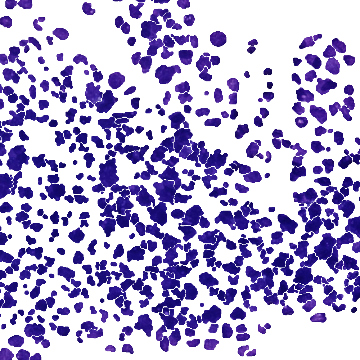
\includegraphics[scale=0.33]{image/aggr_segment_5_masked.png}
	} \\
	\subfigure{
		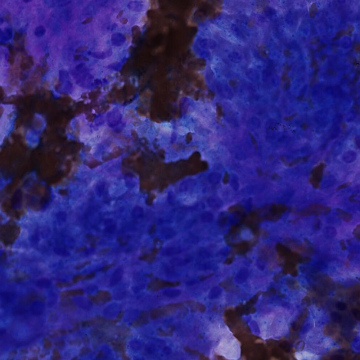
\includegraphics[scale=0.33]{image/aggr_segment_7_in.png}
		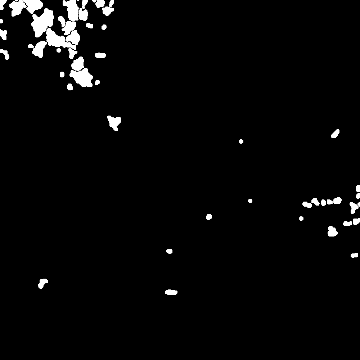
\includegraphics[scale=0.33]{image/aggr_segment_7_out.png}
		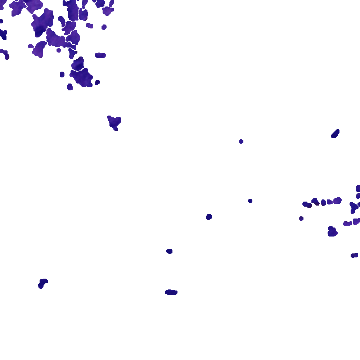
\includegraphics[scale=0.33]{image/aggr_segment_7_masked.png}
	}
	\caption{Examples of aggregate segmentation. See Figure \ref{fig:first_seg_examples} for explanations.}
	\label{fig:second_seg_examples}
\end{figure}

While the presented segmentation procedures exhibit some flaws, they were considered acceptable to test the \textit{SLDC} framework. 

\subsection{Dispatching procedure}
\label{ssec:thyroid_ad_dispatch}

\subsubsection{Slide processing dispatching}

The step (4.4) consists in dispatching detected objects into four categories: artefacts, cells, clusters and patterns. The categories \textit{artefact} and \textit{cluster} respectively correspond to irrelevant objects and to groups of cells that contains too few of them to be patterns. Even if the author distinguishes patterns and clusters at the dispatching step, objects of both categories are treated equally in the subsequent steps of the algorithm. That is, they are first evaluated by the pattern classifier (for assessing whether they are proliferative or not) and they are re-segmented. The dispatching is based on four parameters, the cell minimum and maximum areas (respectively, $A_{min}$ and $A_{max}$), the cell minimum circularity ($C_{min}$) and the minimum number of cells per pattern ($N_{min}$). The values of those parameters as defined by Antoine Deblire are given in Table \ref{tab:adeb_disp_rules}. The dispatching rules can be summarized as follows:

\begin{itemize}
	\item \textbf{Artifact}: all objects having an area less than $A_{min}$ or an area less than $A_{max}$ and a circularity less than $C_{min}$
	\item \textbf{Cell}: all objects having an area $A$ such that $A_{min} < A < A_{max}$ and a circularity greater than $C_{min}$
	\item \textbf{Clusters}: all objects having an area $A$ greater than $A_{max}$ such that the object can contain at most $N_{min}$ cells:
	\[
		A_{max} < A < N_{min} \times A_{max}
	\]
	\item \textbf{Patterns}: all objects which do not match one of the rules above are considered as patterns
\end{itemize}

\begin{table}
	\center
	\begin{tabular}{|c|c|}
		\hline
		$A_{min}$ & 31 $\mu m^2$\\
		\hline
		$A_{max}$ & 102 $\mu m^2$\\
		\hline
		$C_{min}$ & 0.7 \\
		\hline
		$N_{min}$ & 4\\
		\hline
	\end{tabular}
	\caption{Dispatching parameters presented in \cite{adeblire2013}}
	\label{tab:adeb_disp_rules}
\end{table}

In order to find values for those parameters, the author extracted the crops of the cells annotated by the experts, applied to them one of the segmentation procedures presented in Section \ref{ssec:segmentation_proc}, and finally computed the area and circularity of the resulting shapes. While the author does not precise in the thesis which segmentation procedure was applied, it is probably the second (i.e. pattern segmentation). Indeed, as the first was designed to segment both patterns and cells, it would fail at isolating an annotated cell located inside a pattern. While the idea behind this procedure is sound, the geometrical features will probably not be as accurate as expected because of segmentation imperfections. Typical cases when the segmentation fails at providing accurate results are, for instance, cell under-segmentation (see Figure \ref{sfig:area_underseg}) and detection of several objects instead of one. The second case can happen either by splitting a cell in several sub-objects (see Figure \ref{sfig:area_multi}) or because the expert's annotation covers other cells (see Figure \ref{sfig:area_other}). 

\begin{figure}
	\center 
	\subfigure [Under-segmentation] {
		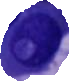
\includegraphics[scale=0.75]{image/area_under_init.png}
		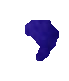
\includegraphics[scale=0.75]{image/area_under_seg.png}
		\label{sfig:area_underseg}
	}
	\hfill
	\subfigure [Detection of several objects] {
		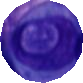
\includegraphics[scale=0.75]{image/area_mult_init.png}
		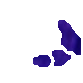
\includegraphics[scale=0.75]{image/area_mult_seg.png}
		\label{sfig:area_multi}
	}
	\hfill
	\subfigure [Detection of another cell included in the mask] {
		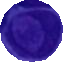
\includegraphics[scale=0.75]{image/area_other_init.png}
		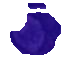
\includegraphics[scale=0.75]{image/area_other_seg.png}
		\label{sfig:area_other}
	}
	\caption{Cases when the segmentation fails at providing accurate results for area and circularity computations. For each example, images to the left and to the right are respectively the original image with a mask representing the annotation shape and the image resulting from the application of the segmentation mask.}
\end{figure}

However, one can assume that the author overcame those issues. Indeed, as stated in the thesis, he generated the circularity and area histograms and then used them to evaluate the thresholds presented in Table \ref{tab:adeb_disp_rules}. However, the author made a mistake in this process as he didn't check whether those thresholds were valid regarding patterns areas and circularities. Especially, are those dispatching rules likely to dispatch cells as patterns or patterns as cells? In order to evaluate this question, the following methodology was applied: crops of annotated patterns and cells were extracted from Cytomine. The former were segmented using the first segmentation and the latter with the second one. For each annotation, the convex hull of the union between the segmented objects was taken as a temporary mask. This operation allows to handle the multi-objects detection problem and also, in some cases, to mitigate the impact of under-segmentation on the resulting area. Finally, in order to make sure that the temporary mask didn't cover areas outside of the expert's annotation, the final mask was generated by taking the intersection between the annotation mask and the temporary mask. This process is illustrated in Figure \ref{fig:annot_cleaning}.

\begin{figure}
	\center
	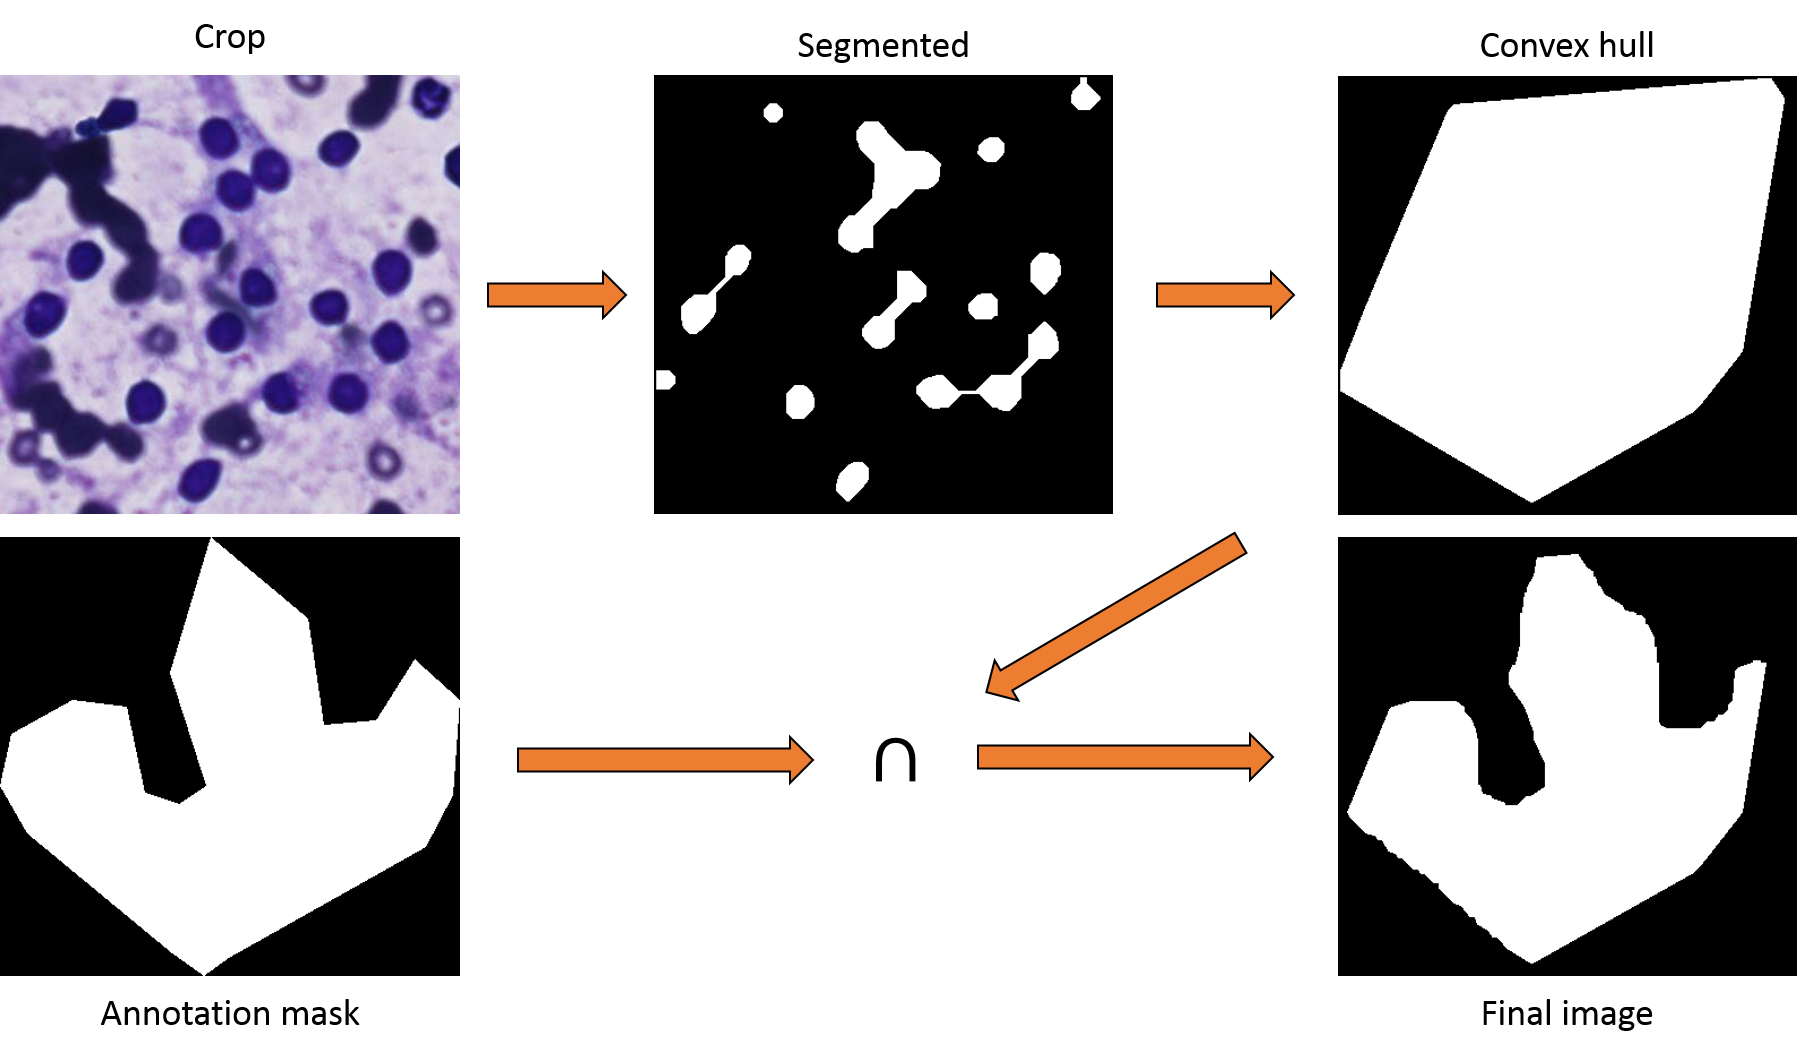
\includegraphics[scale=0.45]{image/area_annot_cleaning.png}
	\caption{Cleaning process for area and circularity assessment.}
	\label{fig:annot_cleaning}
\end{figure}

The histograms given in Figures \ref{fig:hist_area_cell_vs_pattern} and \ref{fig:hist_circ_cell_vs_pattern} respectively show the area and circularity distributions of the segmented experts' annotations. First, it appears that, whatever the metric, there is a substantial overlapping between the cells' and patterns' distributions. This has a major consequence for the dispatching procedure presented above. Indeed, as it relies on simple thresholdings, it is ineffective at separating the objects. Another observation is that the parameters given in Table \ref{tab:adeb_disp_rules} are not relevant as most of the cells would be dispatched as patterns with such values. This observation is confirmed with the scatter plot shown in Figure \ref{fig:scatter_area_circ_cell_vs_pattern}. In this plot, only few cells are effectively dispatched as such (see the blue box in the top left corner of the plot), the others being dispatched as patterns. Given those observations, it is clear that the dispatching procedure must be re-worked.

\begin{figure}
	\center
	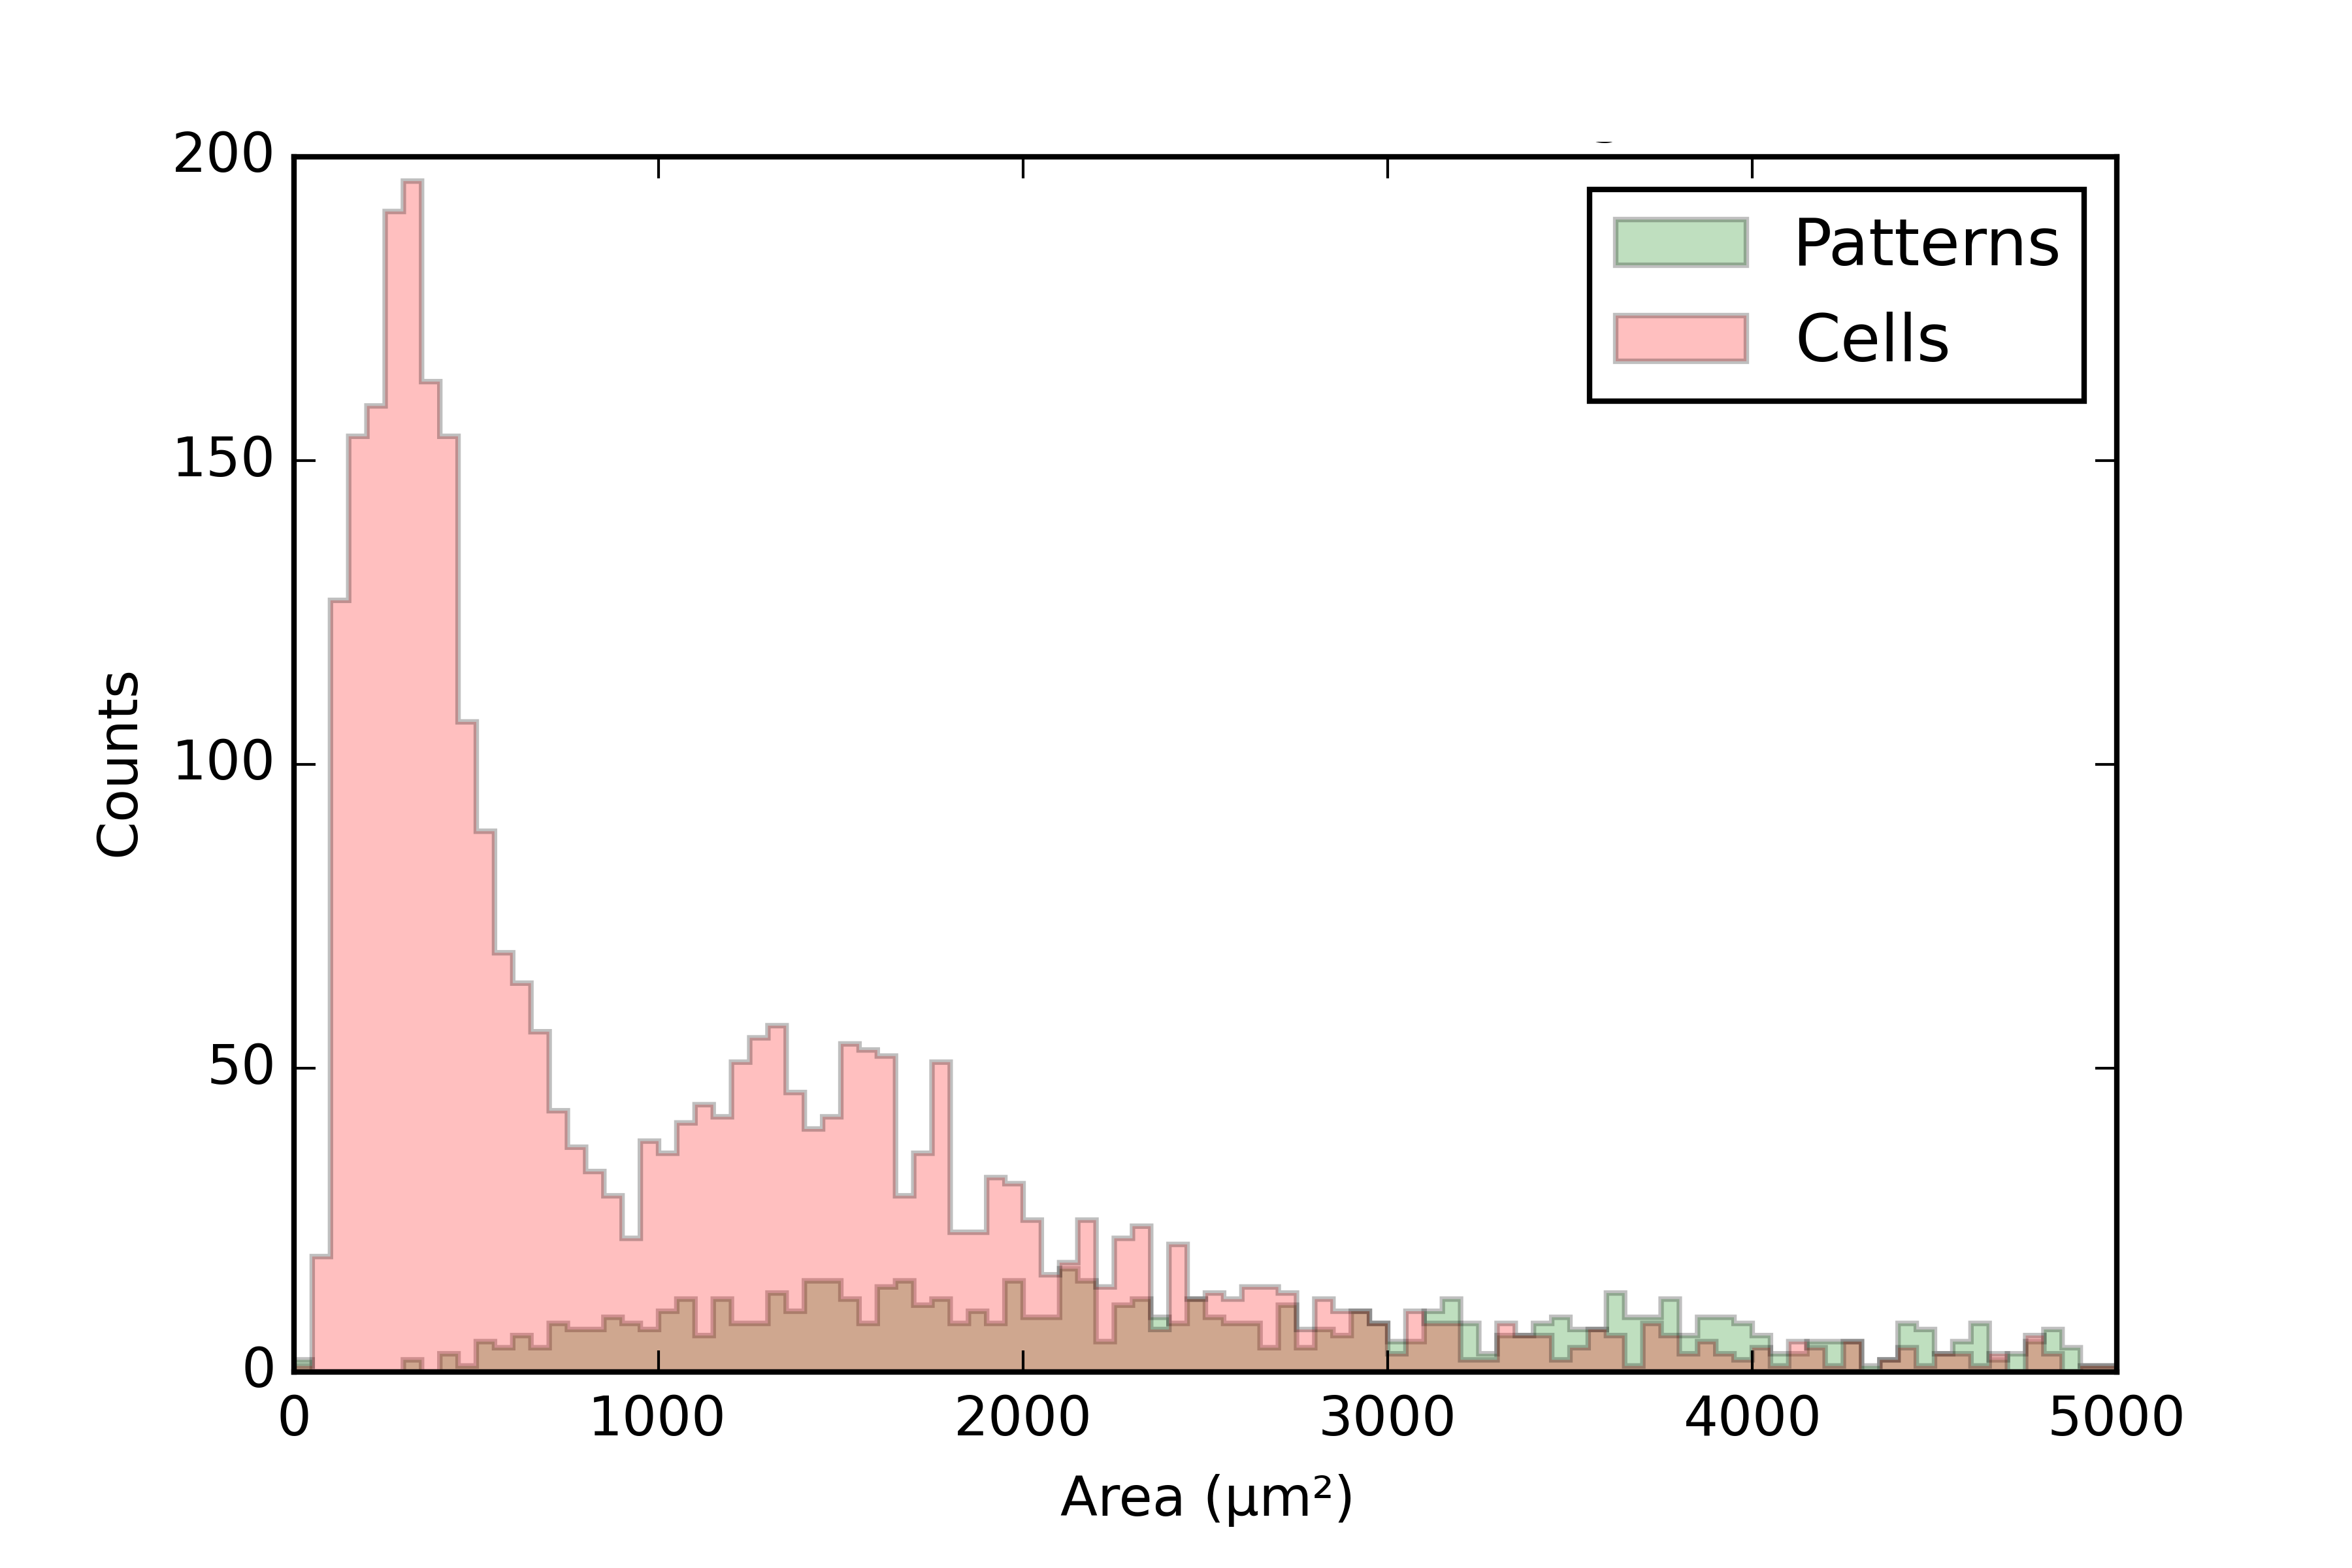
\includegraphics[scale=0.75]{image/cells_patterns_real_area_0_5000.png}
	\caption{Area distributions of the segmented experts' annotations.}
	\label{fig:hist_area_cell_vs_pattern}
\end{figure}

\begin{figure}
	\center
	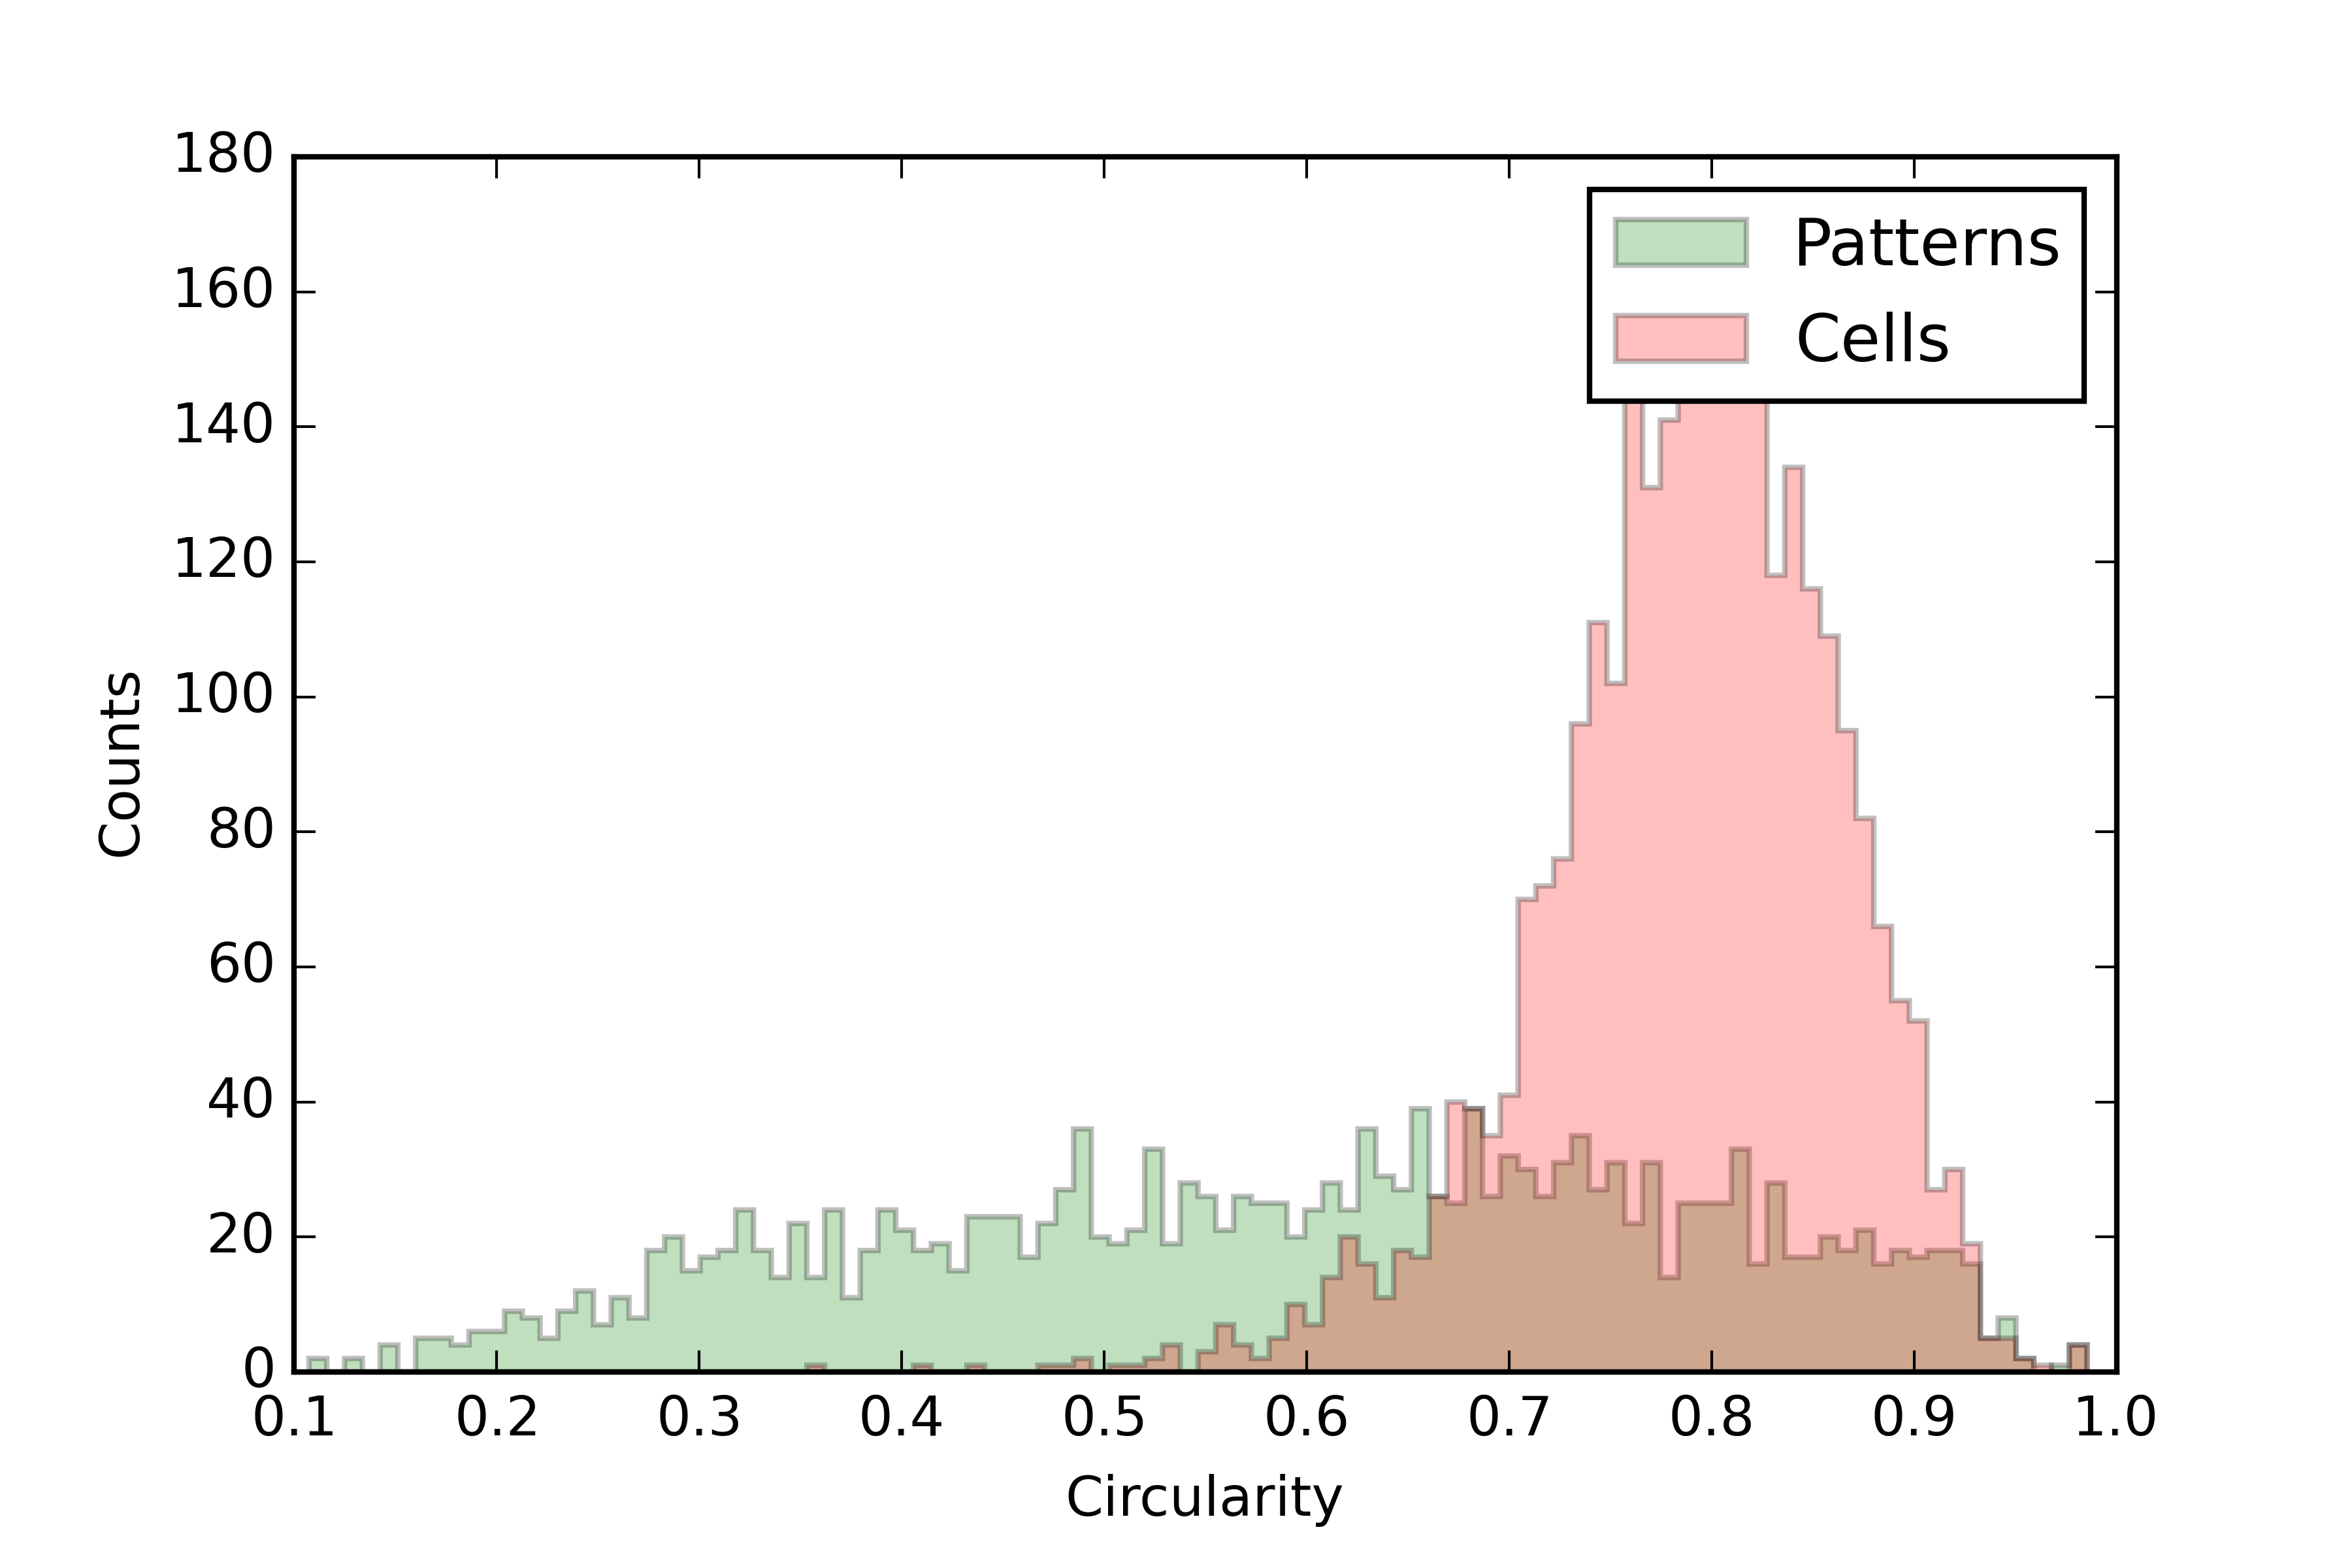
\includegraphics[scale=0.75]{image/cells_patterns_circ.png}
	\caption{Circularity distribution of the segmented experts' annotations.}
	\label{fig:hist_circ_cell_vs_pattern}
\end{figure}


\subsubsection{Improvement}

As relying solely on geometrical properties is not a viable solution, an alternative consists in using the objects' crop image. Especially, the objects' crop would be classified into one of the dispatching categories (i.e. cell, pattern or other) using the random subwindows image classification algorithm \cite{Maree201617} (this algorithm is detailed in Appendix \ref{app:random_subwindows}). A drawback of this solution is that the dimensions of the objects are completely ignored. Given that some patterns might have a similar appearance than cells (color and shape), this might lead to misclassification. 

The avoid the dispatching problem induced by simple thresholdings, one could include the geometrical information of the polygons into the learning and prediction processes. Especially, using the ET-FL variant of the random subwindows algorithm, the area and circularity would be appended to the feature vector generated from the extra-trees classifier. This augmented feature vector would then be passed to the SVM classifier for prediction. While intuitively, this solution seems appealing, it might need to be refined a little more. Indeed, the number of features generated from the extra-trees classifier is relatively large (e.g. for the models presented in Section \ref{ssec:thyroid_perf_models}, this number can reach 30000) and the geometrical features might therefore be overlooked by the SVM classifier. To overcome this problem, a kernel that would increase the contribution of the geometrical features could be used. Whereas this solution might yield better results than the first, it requires the experts' annotations of the learning set to be cleaned to avoid the problem mentioned in Section \ref{sec:thyroid_impl_issue}. Also, it would require a non-negligible modification of the random subwindows algorithm. As the goal is mostly to apply the framework and considering the amount of work implied by this solution, it was considered out of the scope for this thesis and geometrical features were not included among the inputs of the dispatching classifier.

\begin{figure}
	\center
	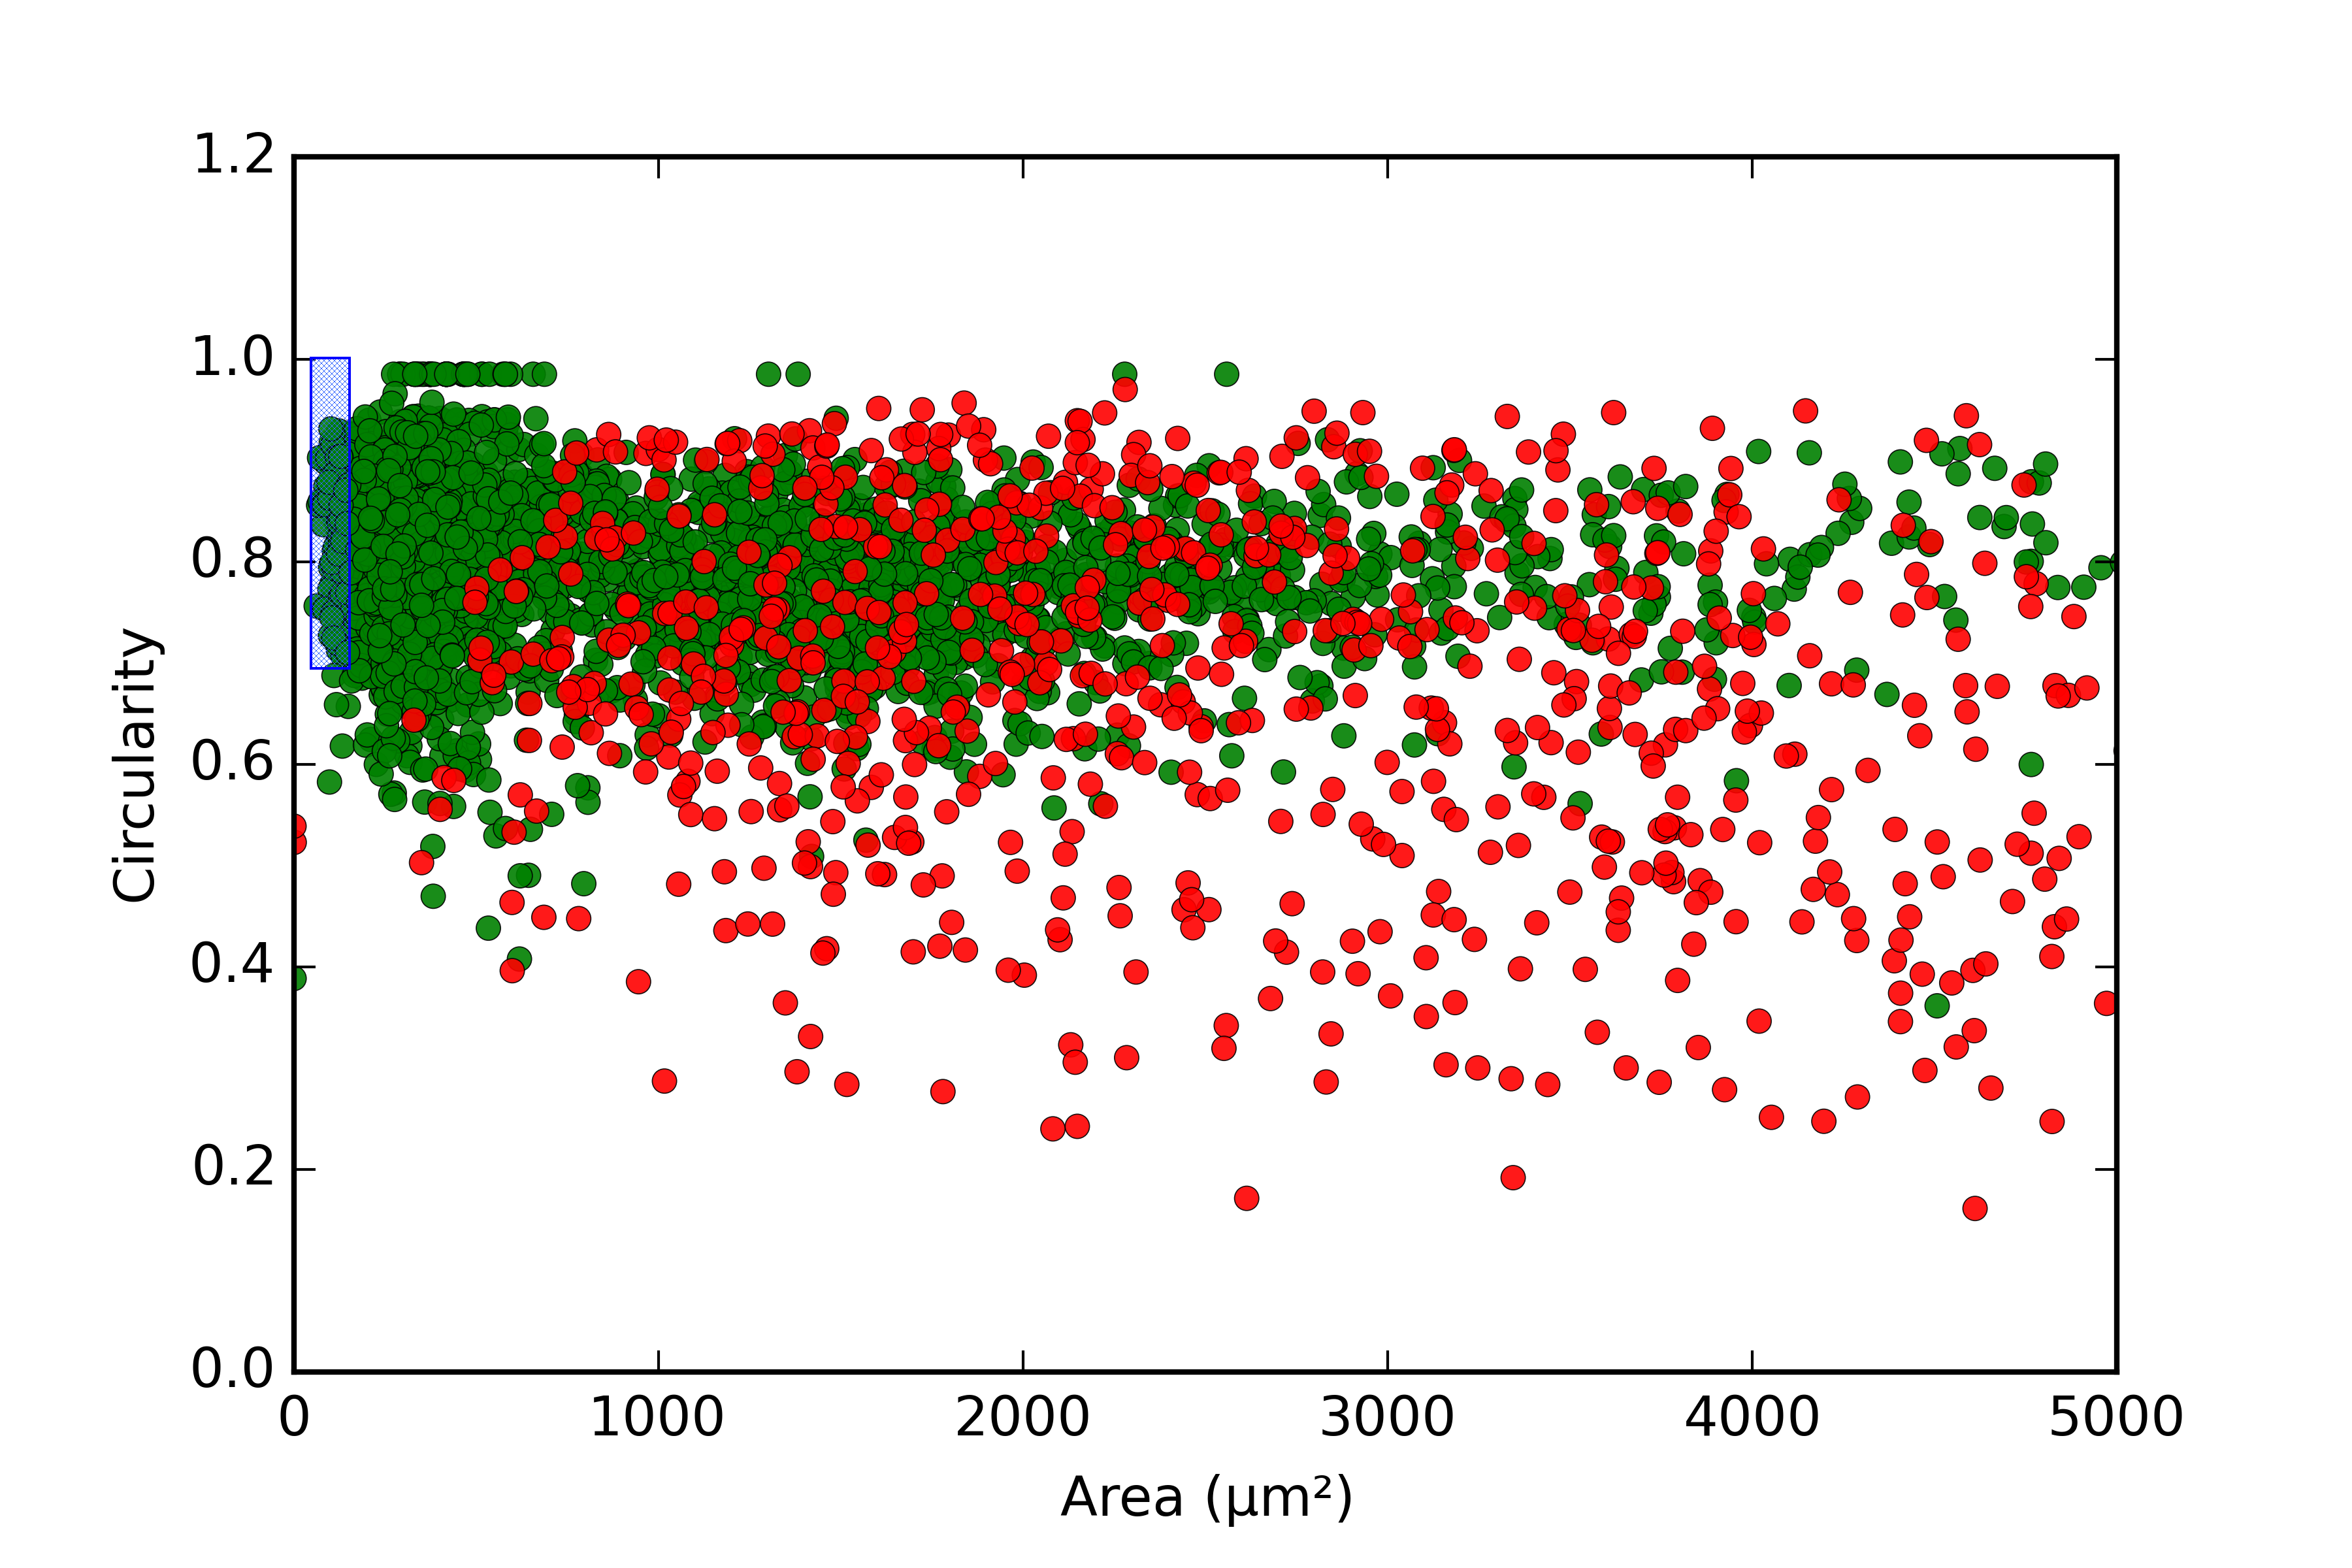
\includegraphics[scale=0.75]{image/scatter_cells_patterns_0_5000.png}
	\caption{Scatter plot, circularity versus area. Green and red dots correspond respectively to cells and patterns. The blue box is the cell dispatching zone.}
	\label{fig:scatter_area_circ_cell_vs_pattern}
\end{figure}

\subsubsection{Pattern processing dispatching}
	
The dispatching strategy designed in \cite{adeblire2013} for the pattern processing phase is simpler. As the objects to be processed by this step are assumed to be cells, the dispatcher filters the detected objects using their geometrical properties. All objects having an area either less than $A_{min}$ or greater than $A_{max}$ or a circularity less than $C_{min}$ are not dispatched the to cell classifier. As explained in previous sections, those parameters are not reliable for dispatching and a new strategy must therefore be defined. It should take into account the flaws of the second segmentation procedure. Especially, it should eliminate the large patches segmented on "\textit{dirty}" patterns. Typically, those are non-spherical (see Figure \ref{fig:second_seg_examples}) and this property can be used to filter them. Moreover, it might be interesting to filter small artefacts and this can be done by filtering objects having a small area. The resulting dispatching rule is the following: every object of which the area is less than $A'$ or of which the circularity is less than $C'$ are removed. Especially, $A'$ was set to $15 \mu m^2$ and $C'$ to $0.6$. It can be seen in Figures \ref{fig:hist_area_cell_vs_pattern} and \ref{fig:hist_circ_cell_vs_pattern} that those thresholds allow to capture almost all cells. 

\subsection{Classification}

As soon as objects are dispatched, they have to be classified. In \cite{adeblire2013}, the author uses two classification models: one for cells and another one for patterns. For patterns, a ternary classifier is used and predicts the following classes: \textit{proliferative pattern}, \textit{non-proliferative pattern} and \textit{other}. The author states that the third class is needed because with a binary classifier, some objects were classified as patterns while they were not patterns. Hopefully, with the new dispatching procedure, those objects will be eliminated before reaching the classifier. It was therefore decided to use a binary classifier for performing this classification. 

As far as the cell classifier is concerned, it predicts two classes: \textit{cells with inclusion} and \textit{non-inclusion}. In addition to the term \textit{cell with inclusion}, the author includes the \textit{pseudo inclusion} in the positive class in order to avoid missing some real inclusions that might look like a pseudo one. 

The final classifiers used for this implementation are detailed in Section \ref{ssec:thyroid_perf_models}.

\section{Implementation}
\label{sec:thyroid_implementation}
Following the \textit{SLDC} framework philosophy, the problem dependent components have to be defined: the image representation, the segmentation procedures, the dispatching rules and the classifiers. Whenever possible, the components were developed to be reusable for other applications within Cytomine. Those generic components are coloured in blue in UML diagrams while the problem dependent components are coloured in green.

\subsection{Image representation}

The first component to be defined is the actual representation of the images to be processed, that is, the digitized microscope slides stored on the Cytomine platform. This representation is implemented in the \texttt{CytomineSlide} class which stores an \texttt{ImageInstance}\footnote{The \texttt{ImageInstance} class is defined in the Cytomine Python client} object containing all the information about the slide including its width, height and identifier. To prevent anyone from loading the full image into memory, the implementation of the \texttt{np\_image} raises a \texttt{NotImplementedError} exception. 

In general, when the full image can be loaded into memory the default \texttt{Tile} class can be used. In this case, as this operation is impossible, a class \texttt{CytomineTile} was created to handle the tile image loading. Especially, the call to \texttt{np\_image} triggers an HTTP request to the Cytomine server to fetch the corresponding image window. If the request fails (e.g. HTTP error) or returns an invalid result (e.g. returned image has an invalid size), a \texttt{TileExtractionError} is raised as advised in the documentation. The class \texttt{CytomineTileBuilder} was created to build \texttt{CytomineTile} objects.

In order to reduce the overall execution time of the workflow, it is essential not to execute two times a HTTP request for loading the same image window. To avoid this, the class \texttt{TileCache} was developed. It implements a simple caching policy using the local file system: when an image window is needed, the \texttt{TileCache} object first checks whether this image was already downloaded and stored on the disk. If that is the case, the request execution is bypassed and the image is loaded from the file. Otherwise, the image is fetched by calling the \texttt{np\_image} method of the underlying tile and stored on the disk before being handed back to the caller. The class also provides methods for adding an alpha mask to the returned image. 

Some additional classes were developed to handle the addition of an alpha mask to an image window (class \texttt{CytomineMaskedWindow}) and to a tile (classes \texttt{CytomineMaskedTile} and \texttt{CytomineMaskedTileBuilder}). This feature is needed for the pattern segmentation procedure which assumes that an alpha mask indicating the position of the pattern is passed with the numpy array. To avoid storing an image representing the alpha mask into memory, the mask is represented by a polygon. 

The UML diagram of the package containing the image-related classes is shown in Figure \ref{fig:uml_cyto_im_repr}.

\begin{figure}
	\center
	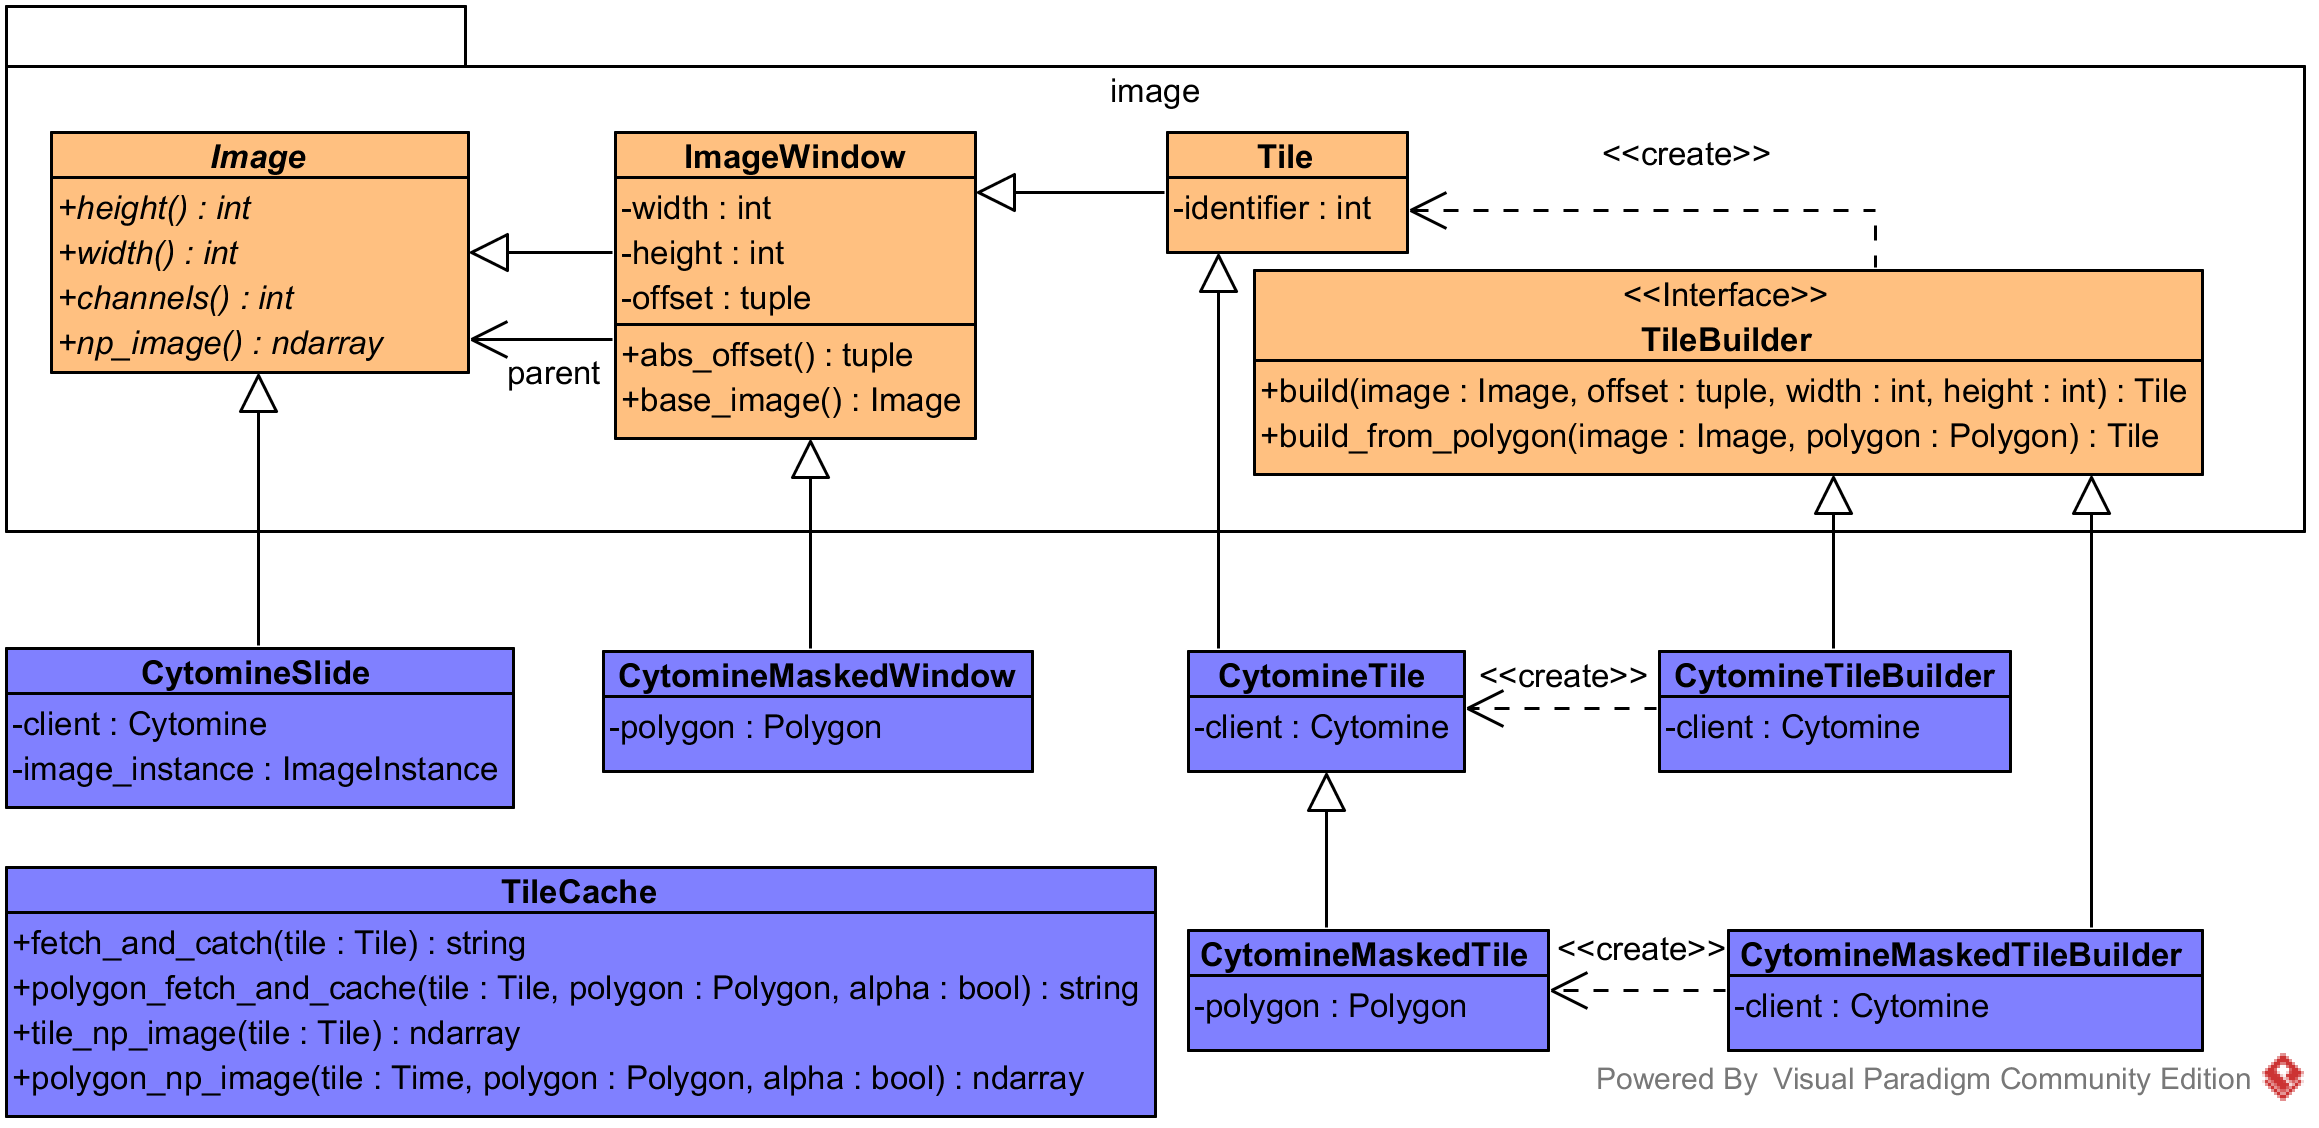
\includegraphics[scale=0.75]{image/thyroid_image.png}
	\caption{UML diagram - Cytomine image representation}
	\label{fig:uml_cyto_im_repr}
\end{figure}

\subsection{Classifier}

In the context of the the thyroid problem, all classification tasks are performed using the random subwindows algorithm \cite{Maree201617}. Especially, a Python implementation called Pyxit taken from Cytomine \cite{maree2016collaborative} was used. The central class of this implementation is the \texttt{PyxitClassifier} class which provides a scikit-learn like interface to the algorithm (i.e. the methods \texttt{fit}, \texttt{transform}, \texttt{predict},...). In order to use this class within the framework, a class \texttt{PyxitClassifierAdapter} was developed. The \texttt{predict\_batch} method is implemented as follows.

 First, the crops of the polygons passed to the method are fetched and stored on the disk using a \texttt{TileCache} (thanks to the cache, the HTTP request is only executed the first time the crops are requested). Because there can be a lot of polygons, the fetching of the crops is parallelized and the number of available processes can be specified at the construction of the \texttt{PyxitClassifierAdapter} object. In order to reduce the serialization overhead, each available process is passed a set of polygons (see Section \ref{sssec:work_parallel}). If some crops cannot be fetched for whatever reason, the corresponding polygons are associated a class \texttt{None} and a probability 0. Moreover the user is notified with the logger about the crops that couldn't be fetched.

As Pyxit works with images stored on the disk, a list containing the filepath of the images to classify is generated and passed to the \texttt{\_predict} method. This method implements the generation of the classification labels and probabilities. If a SVM classifier was provided at construction of the \texttt{PyxitClassifierAdapter} object, then the ET-FL variant of the random subwindows algorithm is used. That is, the Pyxit classifier is used to generate the features that are passed to the SVM classifier for predicting the labels. Otherwise, the variant that uses the extremely randomized trees as direct classifier is used. Finally, the \texttt{predict\_batch} method aggregates the results returned by the \texttt{\_predict} method with the labels and probabilities generated for the polygons of which the crops couldn't be fetched and return those to the caller.

This class also features a static method for constructing a \texttt{PyxitClassifierAdapter} object from a serialized Pyxit model. Especially, the method deserializes the Pyxit classifier as well as the SVM classifier if one is provided and passes them to the adapter's constructor. This method also sets the number of process to use for fetching the crops. If the number of available process is less than five, then all of them are used to fetch the crops. Otherwise, five processes are used at most in order to avoid overloading the Cytomine server.

The UML diagram of the \texttt{PyxitClassifierAdapter} class is shown in Figure \ref{fig:uml_cyto_classifiers}.

\begin{figure}
	\center
	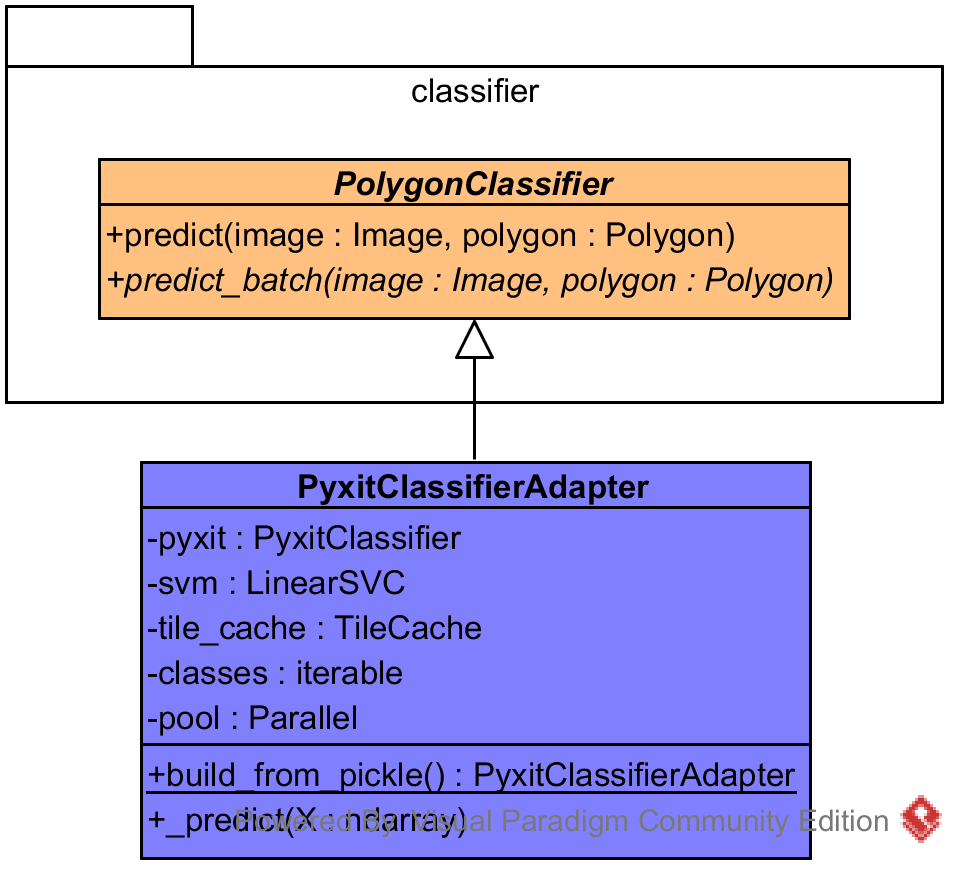
\includegraphics[scale=0.85]{image/thyroid_classifiers.png}
	\caption{UML diagram - Classifier}
	\label{fig:uml_cyto_classifiers}
\end{figure}

\subsection{Dispatching rules}

As explained in Section \ref{ssec:thyroid_ad_dispatch}, the chosen dispatching method relies on a classifier which predicts the dispatching index. Especially, the classifier was built to predict the label 0 for \textit{cell}, 1 for \textit{pattern} and 2 for \textit{other}.

To take advantage of the features provided by the class \texttt{PyxitClassifierAdapter} (i.e. caching, parallel fetching,...), it was reused and encapsulated in two classes extending \texttt{DispatchingRule}. The implementation of the rules' \texttt{evaluate\_batch} method is therefore straightforward. It first calls the \texttt{predict\_batch} method of the classifier adapter object and then generates a list of boolean values according to the returned classification labels. For the first rule, \texttt{CellRule}, \texttt{True} is associated to polygons of which the returned label is 0. For the second, \texttt{AggregateRule}, \texttt{True} is associated with polygons of which the predicted label is 1. After a first run of the algorithm, it appeared that despite the dispatch classifier, a lot small artefacts were dispatched to the cells and patterns classifiers. Therefore, each rule was added a filtering procedure which excludes all objects of which the area is less than a given value. 

Unfortunately, the fact that the dispatching is implemented with two rules implies that the polygons corresponding to patterns and other objects are classified twice. Indeed, because of the dispatching structure imposed by the framework, the polygons that are not matched by the first rule are evaluated by the second. This could be avoided by refactoring the framework or by implementing another dispatching strategy.

The UML diagram containing the dispatching rule classes is shown in Figure \ref{fig:uml_cyto_disp_rules}.

\begin{figure}
	\center
	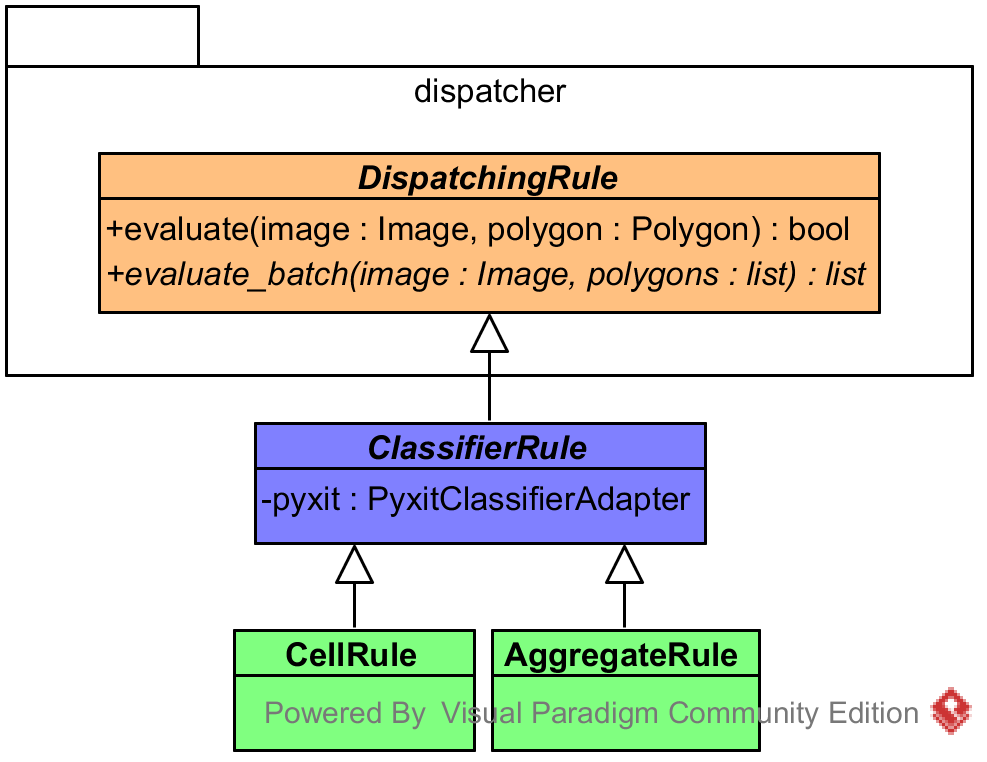
\includegraphics[scale=0.85]{image/thyroid_dispatching_rules.png}
	\caption{UML diagram - Thyroid workflow dispatching rules}
	\label{fig:uml_cyto_disp_rules}
\end{figure}

\subsection{Segmentation}

The segmentation procedures were implemented in two classes, \texttt{SlideSegmenter} and \texttt{AggregateSegmenter}. Both implementation were taken from Antoine Deblire's source code. Whereas the slide segmentation could be used almost directly without modification, the recovered aggregate segmentation procedure did not work. It was therefore re-implemented following the explanations provided in the master thesis as well as the few comments present in the source code. After few tests, it appeared that both segmentation procedures were rather slow because of the color deconvolution. Especially, to execute the color deconvolution on a 4 mega-pixels image yielded more than 2 seconds execution time. A first optimization pass was done over the function in order to reduce its execution time by a factor two. The UML diagram containing the segmenter classes is shown in Figure \ref{fig:uml_cyto_segmenters}.

\begin{figure}
	\center
	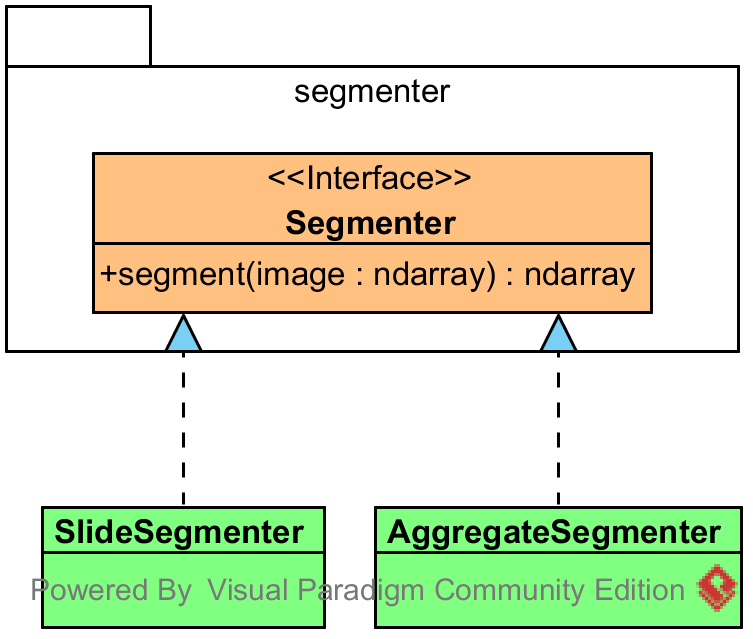
\includegraphics[scale=0.85]{image/thyroid_segmenters.png}
	\caption{UML diagram - Segmenter classes}
	\label{fig:uml_cyto_segmenters}
\end{figure}

\subsection{Chaining}

In order to implement the re-segmentation, the chaining package must be used. First, an image provider must be defined to generate the \texttt{CytomineSlide} objects to be processed. This logic is implemented in the \texttt{SlideProvider} class. Then, the selection of the objects to be processed by the second workflow must be defined as a \texttt{WorkflowExecutor}. Especially, the class \texttt{AggregateWorkflowExecutor} was implemented to fulfill this role. The class defines the method \texttt{get\_windows} which implements the generation of \texttt{CytomineMaskedWindow} objects to be processed by the second workflow. Moreover, it extends the class \texttt{PolygonTranslatorWorkflowExecutor} because the polygons generated by this phase needs to be translated back into the full image reference system. The final component to be defined is the post processor which is passed all the detected objects and their classes. In the context of the thyroid problem, the post processor should upload the generated polygons and classes as annotations on the Cytomine platform. This logic is implemented in the \texttt{post\_process} method of the \texttt{ThyroidPostProcessor} class. Unfortunately, the Cytomine API does not provide any request for uploading annotations by batches and each annotation has to be added with two HTTP requests: one for uploading the geometry and another for uploading the predicted class and associated probability. To avoid waiting for each request to terminate before sending another one, the process was parallelized. The UML diagram containing the chaining classes is shown in Figure \ref{fig:uml_cyto_chaining}.


\begin{figure}
	\center
	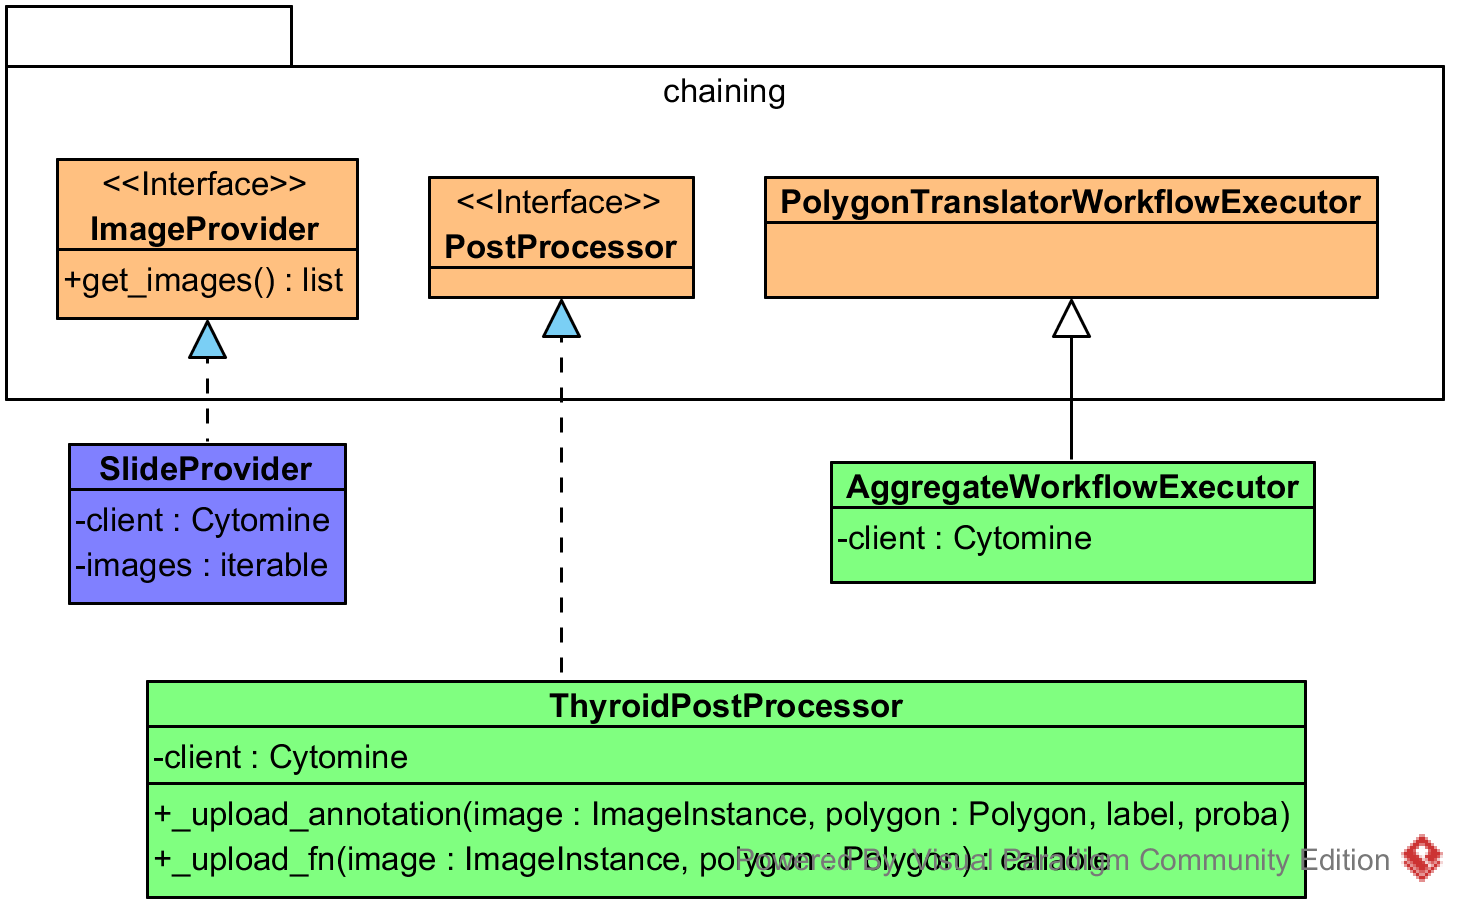
\includegraphics[scale=0.85]{image/thyroid_image_provider.png}
	\caption{UML diagram - Chaining classes}
	\label{fig:uml_cyto_chaining}
\end{figure}


\section{Performance analysis}
\label{sec:thyroid_perf}

\subsection{Classification models}
\label{ssec:thyroid_perf_models}

As explained in Section \ref{sec:thyroid_adeblire_algo}, three classifiers are used by the workflow. The first detects whether an object is a cell, a pattern or another type of object. The second classifies patterns as proliferative or non-proliferative and the last detects whether cells contain an inclusion or not. The roles of these classifiers are illustrated in Figure \ref{fig:summary_classif}. Information about them including the terms associated with the classes, the performances of the models,... are given in Sections \ref{sssec:general_classif}, \ref{sssec:thyroid_pattern_model}, \ref{sssec:thyroid_cell_model} and \ref{sssec:thyroid_disp_model}. Before exploring the classifiers, the methodology followed for assessing the models is presented in Sections \ref{sssec:thyroid_test_set} and \ref{sssec:thyroid_cv}.

\begin{figure}
	\center
	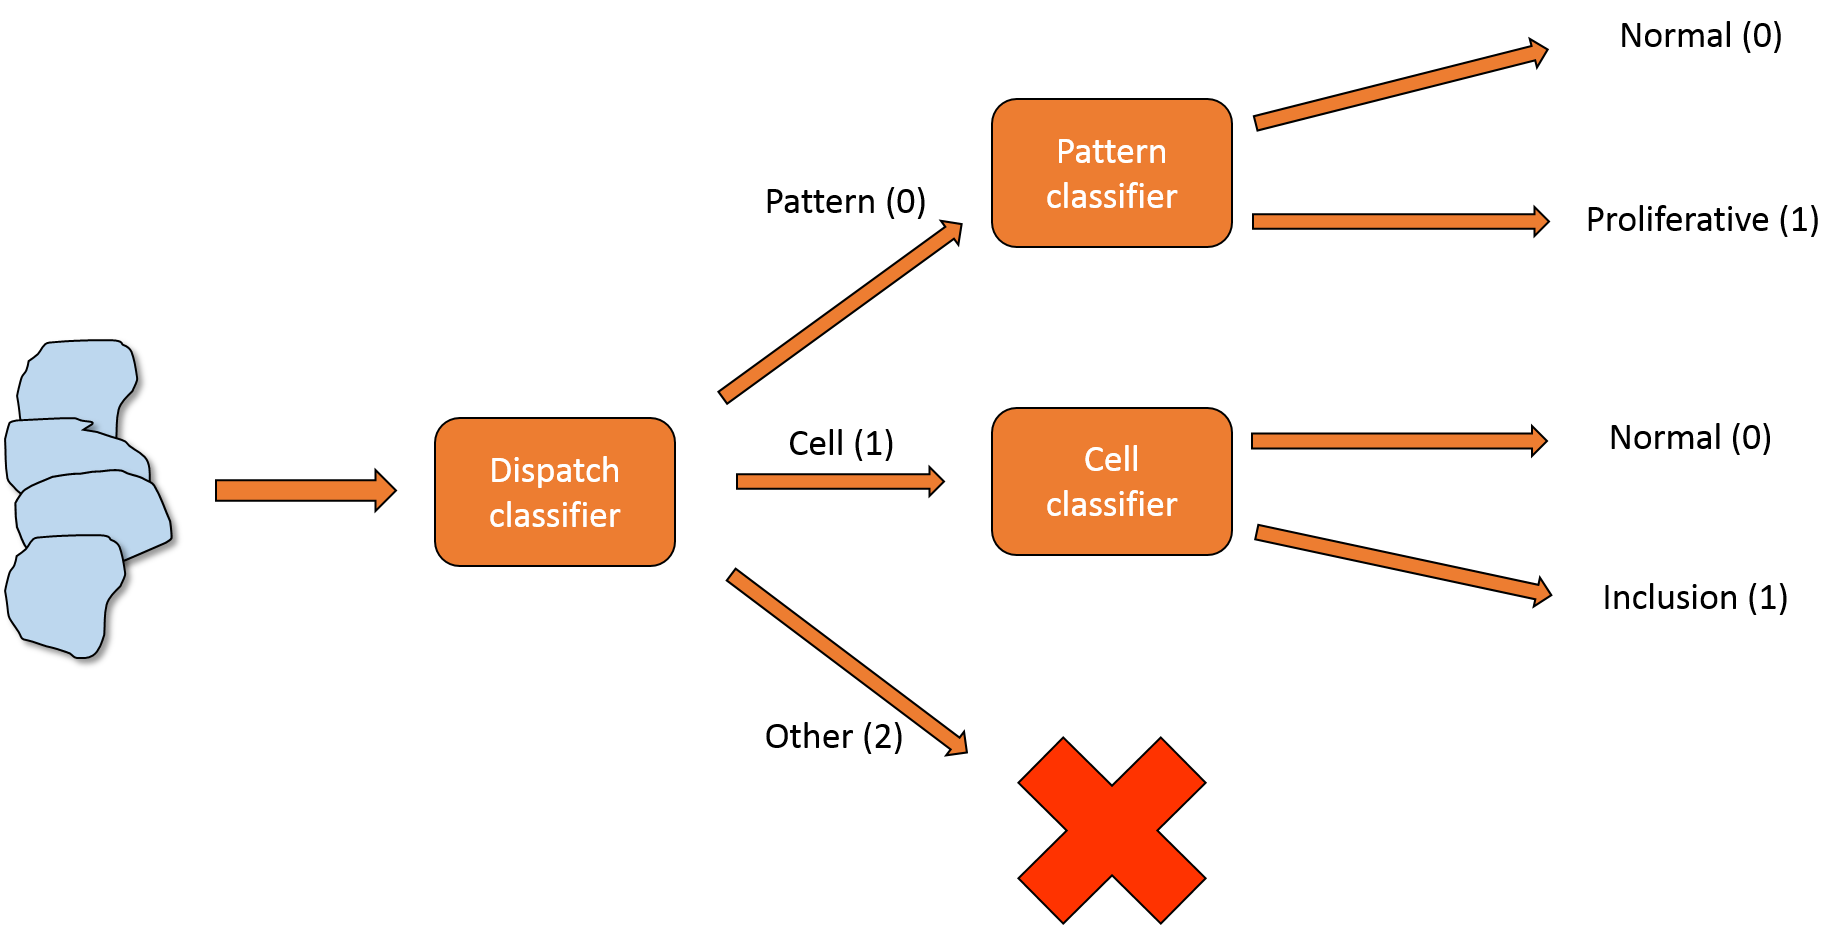
\includegraphics[scale=0.5]{image/summary_classifiers.png}
	\caption{Classifiers' roles summary}
	\label{fig:summary_classif}
\end{figure}

\subsubsection{Test set and metrics}
\label{sssec:thyroid_test_set}
In order to assess a supervised learning model, a classical approach is to split the objects of the input set into a \textit{learning set} on which the model is learned and \textit{test set} on which the error of the model is evaluated. The error extracted using this procedure is called the \textit{generalization error} and is a measure of how accurate the predictions of the model will be on unseen data. Typically, when the number of available objects in the input set is high, a valid splitting strategy consists in leaving approximately 70 \% of the objects in the learning set. The motivation of this proportion is twofold. On the one hand, the learning process have enough data to build relevant models. On the other hand, the test set contains enough samples to make the assessment statistically relevant. However, the proportion is not the only factor that needs to be taken into account. Especially, when the input data is gathered from several sources, the split should be done to avoid overfitting the idiosyncracies of those sources. This can be done by placing the data generated from some sources in the test set and the others into the learning set. Finally, for the assessment to be relevant, both the test and the learning sets should contain instances of all classes. This can be achieved by keeping the target variable's distributions in the learning and test sets close to that of the input set.

The first task performed when it came to build the assessment procedure was therefore to split the input data, namely the experts' annotations, into a test set and a learning set. This was done following the guidelines presented above. Especially, the test set is composed of images selected so that the proportion of annotations it contains is approximately 30 \% and the distribution of the various terms of the ontology is close to their overall distribution in input set. Obviously, satisfying all those constraints at once is impossible given the discrete nature of the problem:

\begin{itemize}
	\item the distributions can only be affected by moving an image into the test set or out of it
	\item each image typically contains between 3 and 10 different terms in different quantity
	\item some terms are contained in very few images. It is particularly true for the \textit{Other} subcategory. For instance, the term "\textit{Macrophage}" is contained in three images only
\end{itemize}

The final split was performed manually. Indeed, due the terms distribution across the images, a random generation was likely to yield a test set in which some terms were missing. The construction process was rather simple: images were taken out from the learning set one after another. When moving an image induced a major imbalance, it was put back into the learning set and another image was taken out instead until an acceptable distribution was reached. The final terms distribution in the test set and learning set is shown in Table \ref{tab:term_distrib}. It can be seen in this table that some terms are slightly imbalanced (e.g. normal cells or artifacts). This is due to the fact that modifying the split to balance those would have broken the balance of more important terms such as cells with inclusion or proliferative patterns. 

\begin{table}
	\small
	\center
	\begin{tabular}{|c|c|cc|cc|cc|cc|}
		\hline
		\multicolumn{2}{|c|}{\multirow{2}{*}{}} &\multicolumn{6}{|c|}{\textbf{Class count and proportions}} & \multicolumn{2}{c|}{\textbf{LS/TS prop.}} \\
		\cline{3-10}
		\multicolumn{2}{|c|}{} & \multicolumn{2}{|c|}{\textbf{Input set}} & \multicolumn{2}{c|}{\textbf{LS}} & \multicolumn{2}{c|}{\textbf{TS}} & \textbf{LS} & \textbf{TS} \\
		\hline
		\multicolumn{2}{|c|}{\textbf{Terms}} & Count & \% & Count & \% & Count & \% & \% & \% \\
		\hline 
		\parbox[t]{2mm}{\multirow{6}{*}{\rotatebox[origin=c]{90}{Cell}}} & NOS & 874 & 14.76 & 567 & 13.85 & 307 & 16.81 & 64.87 & 35.13 \\
		& Normal & 954 & 16.11 & 548 & 13.38 & 406 & 22.23 & 57.44 & 42.56 \\
		& Pseudo-inclusion & 212 & 3.58 & 160 & 3.91 & 52 & 2.85 & 75.47 & 24.53 \\
		& Ground glass & 13 & 0.22 & 8 & 0.20 & 5 & 0.27 & 61.54 & 38.46 \\
		& Grooves & 194 & 3.28 & 144 & 3.52 & 50 & 2.74 & 74.23 & 25.77 \\
		& Inclusion & 738 & 12.46 & 522 & 12.75 & 216 & 11.83 & 70.73 & 29.27 \\
		\hline
		\parbox[t]{2mm}{\multirow{3}{*}{\rotatebox[origin=c]{90}{Pattern}}} & Normal & 798 & 13.48 & 584 & 14.26 & 214 & 11.72 & 73.18 & 26.82 \\
		& Prolif. & 761 & 12.85 & 540 & 13.19 & 221 & 12.10 & 70.96 & 29.04 \\
		& Prolif. (minor)& 300 & 5.07 & 225 & 5.49 & 75 & 4.11 & 75.00 & 25.00 \\
		\hline
		\parbox[t]{2mm}{\multirow{6}{*}{\rotatebox[origin=c]{90}{Other}}} & Macrophage & 273 & 4.61 & 155 & 3.79 & 118 & 6.46 & 56.78 & 43.22 \\
		& Red blood & 98 & 1.66 & 24 & 0.59 & 74 & 4.05 & 24.49 & 75.51 \\
		& Polynuclear & 226 & 3.82 & 177 & 4.32 & 49 & 2.68 & 78.32 & 21.68 \\
		& Colloid & 57 & 0.96 & 37 & 0.90 & 20 & 1.10 & 64.91 & 35.09 \\
		& Artefact & 286 & 4.83 & 281 & 6.86 & 5 & 0.27 & 98.25 & 1.75 \\
		& Background & 137 & 2.31 & 123 & 3.00 & 14 & 0.77 & 89.78 & 10.22 \\
		\hline
		& \textbf{Total} & \textbf{5921} & 100 & \textbf{4095} & 100 & \textbf{1826} & 100 & \textbf{70.49} & \textbf{29.51} \\
		\hline
		\multicolumn{2}{|c|}{\textbf{Images}} & \multicolumn{2}{|c|}{61} & \multicolumn{2}{c|}{43} & \multicolumn{2}{c|}{18} & &  \\
		\hline
	\end{tabular}
	\caption{Terms distribution in the learning set and test set.}
	\label{tab:term_distrib}
\end{table}

Now that the test set is built, the metrics that will be used for assessing the models must be defined. In classification, the most common is the \textit{accuracy} which is the proportion of correctly classified objects. In the particular case of binary classification (the target is either positive or negative), two common metrics are:

\begin{itemize}
	\item \textbf{recall}: the number of true positive over the number of positive. Intuitively, it is the ability of the classifier to find the positive objects. 
	\item \textbf{precision}: the number of true positive over the number of predicted positive. Intuitively, it is the ability of the classifier not to classify positive objects as negative.
\end{itemize}

All the previous metrics can be computed based the confusion matrix, a square matrix of order $N$ where $N$ is the number of classification labels. Its element $m_{ij}$ contains the number of objects that are actually associated the $i^{th}$ label but were predicted the $j^{th}$ one by a model. In order to have several indicators of the models performances, all the metrics mentioned above were used. 

\subsubsection{Cross validation and model selection}
\label{sssec:thyroid_cv}
The random subwindows algorithm has several parameters that can be tuned to improve the model performances. It includes the parameters of the underlying classifier such as the minimum number of objects required to split a node or the maximum number of features to evaluate when looking for the best split in the decision tree algorithm. The algorithm has also proper parameters such as the minimum and maximum sizes of the windows to extract or the colorspace into which the windows must be converted before being passed to the underlying classifier. The complete list of parameters is given in Table \ref{tab:tunable_parameters}. 

\begin{table}
	\small
	\center
	\begin{tabular}{|c|c|p{0.35\linewidth}|}
		\hline
		\textbf{Name} & \textbf{Classifier} & \textbf{Description} \\
		\hline
		\texttt{pyxit\_min\_size} & Pyxit & Minimum size proportion of the windows to extract (relative to the full image size). \\
		\texttt{pyxit\_max\_size} & Pyxit & Maximum size proportion of the windows to extract (relative to the full image size). \\
		\texttt{colorspace} & Pyxit & Colorspace into which the windows must be converted before being passed to the underlying classifier. Available colorspaces are HSV and normalized RGB\\
		\texttt{min\_sample\_split} & Extra-trees & Minimum number of objects required to split a node \\
		\texttt{max\_features} & Extra-trees & Maximum number of features to evaluate when looking for the best split in the decision tree algorithm \\ 
		\texttt{C} & SVM & SVM penalty parameter. Only available when the ET-FL variant of the random subwindows algorithm is used.\\
		\hline
	\end{tabular}
	\caption{Random subwindows algorithm parameters to tune}
	\label{tab:tunable_parameters}
\end{table}

In order to maximize the performances of the produced models, a tuning procedure was implemented to extract the best combination of parameters. The procedure creates a set of models using all the possible combinations of parameters values provided by the user. Each model is then assessed using cross-validation and the best parameters are returned. Similarly to model assessment, the fact that annotations come from several images should be taken into account to avoid overfitting. Especially, the performance of a model were assessed using a cross-validation strategy called \textit{leave one image out}. Given a learning set containing $N$ images, each image is taken out from the learning set in turn and the model is learned on the $N - 1$ remaining images. The performance score of the model is then computed on the taken out image. This process generates $N$ scores which are averaged and the resulting score is associated to the model. This process is illustrated in \ref{fig:loio}.

\begin{figure}
	\center
	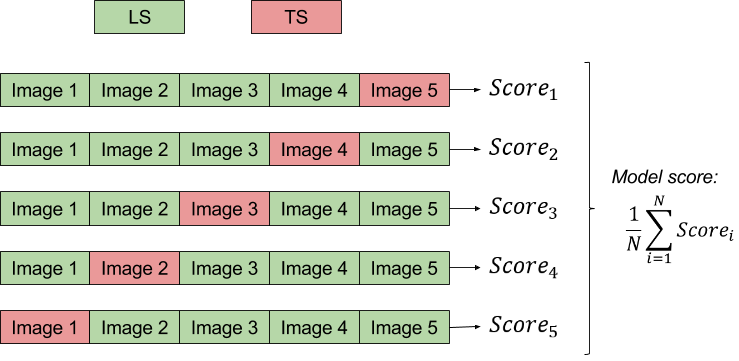
\includegraphics[scale=0.5]{image/leave_one_image_out.png}
	\caption{Leave one image out cross-validation strategy (number of images $N = 5$)}
	\label{fig:loio}
\end{figure}

Finally, the full assessment procedure consists in splitting the dataset into a learning set and a test set. Then, the best parameters are determined by cross-validation on the learning set, a model is learned on the whole learning set with the best parameters and this model is assessed on the test set using the metrics presented in \ref{sssec:thyroid_test_set}.

\subsubsection{General comments about classifiers}
\label{sssec:general_classif}
For each required classifier, both variants of the random subwindows algorithm were evaluated: the first variant where the extra-trees are used as direct classifier (\textit{ET-DIC}), and the second where they are used as features learner to be fed to a SVM classifier (\textit{ET-FL}). Moreover, both variants were evaluated on a first learning set containing only experts' annotations and on a second which was augmented with some reviewed annotations (see Section \ref{sssec:detect_cytomine} for reviewing). Especially, the latter annotations were generated by an execution the workflow on an image from the learning set and  were reviewed on Cytomine in an attempt to improve the classifiers performances. 

As far as the parameters are concerned, a first cross-validation procedure was applied to narrow the search space. Especially, this was applied for finding the ranges in which the window minimum and maximum sizes should be taken. As explained in \cite{Maree201617}, small subwindows yield better results on images containing highly repeatable patterns (e.g. architectural patterns) because they allow to capture fine details. In contrast, larger windows works best on images in which the shape is prevailing (e.g. cells). This intuition was confirmed by a first cross-validation procedure as the best models for classifying cells were built using large windows while small windows yielded better results for classifying patterns.

For the ET-FL variant, the parameter \texttt{min\_sample\_split} was not tuned. Indeed, as suggested in \cite{Maree201617}, it could be set to $\frac{W}{1000}$ where $W$ is the number of subwindows in the learning set. Particularly, this value prevents the extra-trees to learn features that are too specific and also reduces the execution time compared to that of a model for which the parameter was set to $1$. Indeed, the former model contains less leaf nodes which reduces the size of the features vector passed to the SVM classifier. As far as the ET-DIC variant is concerned, the same parameters was tuned with the following set of values: $\left\{1, \frac{W}{1000}, \frac{W}{100}, \frac{W}{50}, \frac{W}{20} \right\}$.

The parameter \texttt{max\_features} was tuned whatever the variant and the same four values were always provided: $\left\{1, \sqrt{M}, \frac{M}{2}, M\right\}$ where $M$ is the number of features passed to the underlying extra-trees classifier. As the dimensions of the resized windows are $16\times 16$, the number of features $M$ equals 768 in this case. Those four values were chosen to span over the range $[1, 768]$ and $\sqrt{M}$ is the default value suggested in \cite{Geurts2006}. 

\subsubsection{Pattern classifier}
\label{sssec:thyroid_pattern_model}
The pattern classifier is a binary model which predicts whether a pattern is proliferative or not. The correspondence between the output classes and the terms of the ontology is rather straightforward and is the following:

\begin{itemize}
	\item Output \textbf{positive} (class 1): 
	\begin{itemize}
		\item \textit{proliferative architectural pattern}
		\item \textit{proliferative architectural pattern (minor sign)}
	\end{itemize}
	\item Output \textbf{negative} (class 0): 
	\begin{itemize}
		\item \textit{normal follicular architectural pattern}
	\end{itemize}		
\end{itemize}

The only terms used are the ones from the subcategory \textit{Pattern} as all the objects to be classified by this model are expected to be patterns.  Indeed, other objects have normally been filtered by the dispatch classifier. Luckily, this distribution of terms yields some rather balanced learning set and test sets (see Table \ref{tab:pattern_classif_dataset_size}). As patterns are usually large objects, only small window sizes were evaluated during cross validation. All the evaluated parameters are given in Appendix \ref{app:cross_val} while the one which yielded the better models are given in Table \ref{tab:pattern_classif_best_params}. It seems that the HSV colorspace is particularly well suited to the pattern classification problem. 

The best models' performances are given in Table \ref{tab:pattern_classif_best_scores} and \ref{tab:pattern_classif_conf_mat}. All models perform relatively well. Especially, almost all models exhibit an impressive recall of 96 \% except for the ET-FL variant with reviewed annotations of which the recall drops to 94 \%.

As the performances are comparable, the model selected to be used for executing the workflow was the ET-DIC variant without reviewed annotations. Especially, it was preferred because it executes faster than the ET-FL variant (see in Section \ref{sssec:perf_first_test_serie}) and also because the model can generate class probabilities.

\begin{table}
	\small
	\center
	\subfigure [Experts' annotations] {
		\begin{tabular}{|c|cc|cc|cc|cc|}
			\hline
			& \multicolumn{2}{|c|}{Prolif.} & \multicolumn{2}{c|}{Normal} & \multicolumn{2}{c|}{Total}\\
			\hline		
			LS & 765 & \tiny (56.71\%) & 584 & \tiny (43.29\%) & 1349 & \tiny (72.57\%)\\
			TS & 296 & \tiny (58.04\%) & 214 & \tiny (41.96\%) & 510 & \tiny (27.43\%)\\
			\hline
			Total & 1061 & \tiny (57.07\%) & 798 & \tiny (42.93\%) & \multicolumn{2}{c|}{}\\
			\hline
		\end{tabular}
	}
	\subfigure [Reviewed] {
		\begin{tabular}{|c|cc|cc|cc|cc|}
			\hline
			& \multicolumn{2}{|c|}{Prolif.} & \multicolumn{2}{c|}{Normal} & \multicolumn{2}{c|}{Total}\\
			\hline		
			LS & 908 & \tiny (60.09\%) & 603 & \tiny (39.91\%) & 1511 & \tiny (74.76\%)\\
			TS & 296 & \tiny (58.04\%) & 214 & \tiny (41.96\%) & 510 & \tiny (25.24\%)\\
			\hline
			Total & 1061 & \tiny (57.07\%) & 798 & \tiny (42.93\%) & \multicolumn{2}{c|}{}\\
			\hline
		\end{tabular}
	}
	\caption{Pattern classifier. Dataset size.}
	\label{tab:pattern_classif_dataset_size}
\end{table}

\begin{table}
	\small
	\center 
	\begin{tabular}{|c|c|cc|cc|}
		\hline
		& & ET-DIC & ET-DIC (r) & ET-FL & ET-FL (r) \\
		\hline
		LS & accuracy & 0.8285 & 0.8224 & 0.8849 & 0.886\\
		\hline
		\multirow{3}{*}{TS} & accuracy & 0.8664 & 0.8468 & 0.8664 & 0.8625\\
		& recall & 0.9662 & 0.9628 & 0.9628 & 0.9493\\
		& precision & 0.8314 & 0.8097 & 0.83333 & 0.8363\\
		\hline
	\end{tabular}
	\caption{Pattern classifier. Best model's performance.}
	\label{tab:pattern_classif_best_scores}
\end{table}

\subsubsection{Cell classifier}
\label{sssec:thyroid_cell_model}

The cell classifier is a binary model which predicts whether a cell contains an inclusion or not. As there are more terms related to cells, the correspondence between the terms of the ontology and the classification labels is slightly more complex than for the pattern classifier:

\begin{itemize}
	\item Output \textit{positive} (class 1): 
	\begin{itemize}
		\item \textit{cell with inclusion}
	\end{itemize}
	\item Output \textit{negative} (class 0): 
	\begin{itemize}
		\item \textit{cell with NOS}
		\item \textit{pseudo-inclusion}
		\item \textit{ground glass nuclei}
		\item \textit{nuclear grooves}
		\item \textit{normal cell}
		\item \textit{red blood cell}
		\item \textit{polynuclear}
	\end{itemize}
\end{itemize}

While for the pattern classifer, only objects from the \textit{Pattern} subcategory were used, the cell classifier is trained with two terms from the \textit{Other} subcategory. This was done because those two terms (i.e. red blood cell and polynuclear) corresponds to objects that can be mistaken with actual cells. Especially, if those objects are dispatched to the cell classifier, it has to be able to associate to them the negative class. Choosing this mapping has nevertheless the drawback of emphasizing the class imbalance. Table \ref{tab:cell_classif_dataset_size} shows that only 25 \% of the objects input set are cells with inclusion. For this classifier, the windows sizes were chosen relatively big (see Table \ref{tab:app_cell_classif_tuned}) as the cells are small objects with few details and no repeatable patterns. 

The performance expectations for this classifier are the following: the consequences of the presence of cells with inclusion is such that those should not be missed. Especially, recall should be as high as possible. Moreover, as the cells found by the workflow would in practice be reviewed by physicians (before making a diagnosis), the number of false positive should also kept as small as possible. This would be expressed by a high precision. The best models' performances are given in Table \ref{tab:cell_classif_best_scores} and \ref{tab:cell_classif_conf_mat}. Those results show that the models do not meet the expectations. Indeed, whereas they exhibit a relatively good precision, the recall is far from being acceptable which indicates that the models fail at detecting cells with inclusion. The performances are particularly bad and worse than random guessing when the model is built using the ET-DIC variant as only 13 \% of the cells with inclusion are correctly labelled as such. The results are better with the ET-FL variant as the recall rises to 50 \% on the dataset containing the reviewed annotations. While the increase is spectacular, the model still performs very poorly as random guessing would yield approximately the same recall. 

Those poor performances might be explained by two elements. The first is the similarity between the cells containing an inclusion and some cells of the negative class. For instance, the cells with pseudo inclusion are very similar to cells with inclusion as shown in Figure \ref{fig:similarity_incl_pseudo}. The second is the class imbalance in the dataset. It appears that adding the reviewed annotations in the learning has improved the recall with the ET-FL variant. Therefore, increasing the amount of data by performing more reviewing might be a solution to improve the classifier. 

Because it exhibits the best recall score, the model ET-FL with reviewed annotations should be used within the workflow.

\begin{figure}
	\center
	\subfigure [Pseudo-inclusion] {
		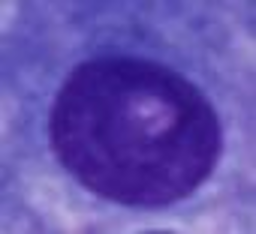
\includegraphics[scale=0.25]{image/pseudo1.png}
		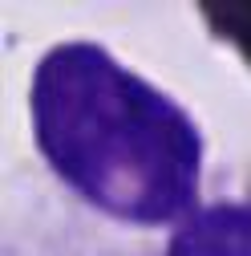
\includegraphics[scale=0.25]{image/pseudo2.png}
		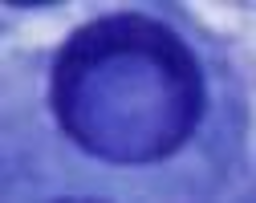
\includegraphics[scale=0.25]{image/pseudo3.png}
		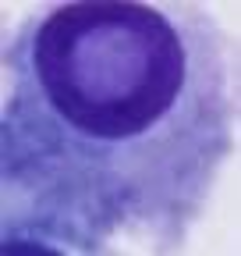
\includegraphics[scale=0.25]{image/pseudo4.png}
	}
	\subfigure [Inclusion] {
		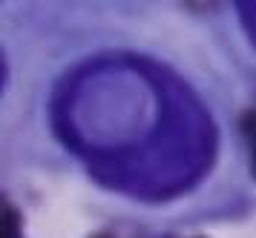
\includegraphics[scale=0.25]{image/incl1.png}
		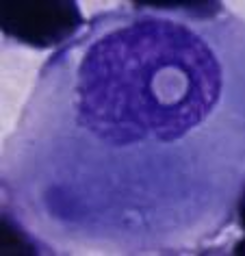
\includegraphics[scale=0.25]{image/incl2.png}
		\includegraphics[scale=0.25]{image/incl3.png}
		\includegraphics[scale=0.25]{image/incl4.png}
	}
	\caption{Similarity between pseudo-inclusion and cells with inclusion}
	\label{fig:similarity_incl_pseudo}
\end{figure}
\begin{table}
	\small
	\center
	\subfigure [Experts' annotations] {
		\begin{tabular}{|c|cc|cc|cc|}
			\hline
			& \multicolumn{2}{|c|}{Inclusion} & \multicolumn{2}{c|}{Normal} & \multicolumn{2}{c|}{Total}\\
			\hline		
			LS & 567 & \tiny (26.37\%) & 1583 & \tiny (73.63\%) & 2150 & \tiny (64.97\%)\\
			TS & 307 & \tiny (26.49\%) & 852 & \tiny (73.51\%) & 1159 & \tiny (35.03\%)\\
			\hline
			Total & 874 & \tiny (26.41\%) & 2435 & \tiny (73.59\%) & \multicolumn{2}{c|}{}\\
			\hline
		\end{tabular}
	}
	\subfigure [Reviewed] {
		\begin{tabular}{|c|cc|cc|cc|}
			\hline
			& \multicolumn{2}{|c|}{Inclusion} & \multicolumn{2}{c|}{Normal} & \multicolumn{2}{c|}{Total}\\
			\hline		
			LS & 571 & \tiny (18.26\%) & 2556 & \tiny (81.74\%) & 3127 & \tiny (72.96\%)\\
			TS & 307 & \tiny (26.49\%) & 852 & \tiny (73.51\%) & 1159 & \tiny (27.04\%)\\
			\hline
			Total & 878 & \tiny (20.49\%) & 3408 & \tiny (79.51\%) & \multicolumn{2}{c|}{}\\
			\hline
		\end{tabular}
	}
	\caption{Cell classifier. Dataset size.}
	\label{tab:cell_classif_dataset_size}
\end{table}

\begin{table}
	\small
	\center 
	\begin{tabular}{|c|c|cc|cc|}
		\hline
		& & ET-DIC & ET-DIC (r) & ET-FL & ET-FL (r) \\
		\hline
		LS & accuracy & 0.7645 & 0.7613 & 0.7813 & 0.7873\\
		\hline
		\multirow{3}{*}{TS} & accuracy & 0.8333 & 0.8351 & 0.8696 & 0.8523\\
		& recall & 0.1302 & 0.1349 & 0.4512 & 0.4930 \\
		& precision & 0.8235 & 0.8529 & 0.7462 & 0.6310 \\
		\hline
	\end{tabular}
	\caption{Cell classifier. Best model's performance.}
	\label{tab:cell_classif_best_scores}
\end{table}

\subsubsection{Dispatching classifier}
\label{sssec:thyroid_disp_model}
The dispatching classifier is a ternary model which predicts whether an object is a cell, a pattern or another type of object. The correspondence between the classes and the terms of the ontology is the following:

\begin{itemize}
	\item Output \textit{pattern} (class 0): 
	\begin{itemize}
		\item \textit{proliferative architectural pattern}
		\item \textit{proliferative architectural pattern (minor sign)} 
		\item \textit{normal follicular architectural pattern}
	\end{itemize}
	\item Output \textit{cell} (class 1): 
	\begin{itemize}
		\item \textit{cell with NOS}
		\item \textit{pseudo-inclusion}
		\item \textit{ground glass nuclei}
		\item \textit{nuclear grooves}
		\item \textit{normal cell}
		\item \textit{red blood cell} 
		\item \textit{cell with inclusion}
	\end{itemize} 
	\item Output \textit{other} (class 2): 
	\begin{itemize}
		\item \textit{background}
		\item \textit{artefact}
		\item \textit{macrophage}
		\item \textit{polynuclear}
		\item \textit{colloid}
	\end{itemize} 
\end{itemize}

Mostly, the correspondence is expected. The only peculiarity is the association of the term \textit{Red blood cell} with the second output. Whereas this term is in the \textit{Other} subcategory, red blood cells look quite much like cells with inclusion. So it seemed a good idea to bias the model so that it redirects those to the cell classifier in order not to miss cells with inclusion. 

As shown in Table \ref{tab:dispatch_classif_dataset_size}, the terms distribution induces an imbalance. The third class is particularly under-represented. However, the imbalance is not as critical as for the cell classifier. As far as the windows dimensions are concerned, the first cross-validation revealed that using both small and large ones at the same time yielded better results (see Table \ref{tab:dispatch_classif_best_params} for the dimensions).

The best models' performances are given in Table \ref{tab:dispatch_classif_best_scores} and \ref{tab:dispatch_classif_conf_mat}. A first observation is that all models seem to be relatively good at dispatching cells and patterns. However, they fail at dispatching other objects. This is particularly true for the ET-DIC variant without reviewed annotations which classifies all the other objects as cells or patterns. The addition of reviewed annotations brings a slight improvement as 4 \% of the other objects are classified as such.

The ET-FL variant brings a non-negligible improvement as for the classification of other objects as 46 \% of them are correctly classified. This model also classifies the patterns more precisely as only 4 \% are misclassified against 11 \% with the ET-DIC variant. Those improvements come at the the cost of a slight degradation of cell classification as 5 \% of them are classified as other objects. The addition of the reviewed annotations (which contain a majority of other objects, see Table \ref{tab:dispatch_classif_dataset_size}) increases the proportion of correctly classified other objects which reaches almost 60 \%. Again, this comes at the cost increasing the misclassification rate for the other classes which reaches approximately 8 \% for both of them.

As it exhibits the best accuracy, the ET-FL variant without reviewed annotations should be used within the workflow to dispatch cells.

\begin{table}
	\small
	\center
	\subfigure [Experts' annotations] {
		\begin{tabular}{|c|cc|cc|cc|cc|}
			\hline
			& \multicolumn{2}{|c|}{Pattern} & \multicolumn{2}{c|}{Cell} & \multicolumn{2}{c|}{Other} & \multicolumn{2}{c|}{Total}\\
			\hline		
			LS & 1349 & \tiny (32.94\%) & 1973 & \tiny (48.18\%) & 773 & \tiny (18.88\%) & 4095 & \tiny (69.16\%)\\
			TS & 510 & \tiny (27.93\%) & 1110 & \tiny (60.79\%) & 206 & \tiny (11.28\%) & 2435 & \tiny (30.84\%)\\
			\hline		
			Total & 1859 & \tiny (31.4\%) & 3083 & \tiny (52.07\%) & 979 & \tiny (0.1653\%) & \multicolumn{2}{c|}{}\\
			\hline
		\end{tabular}
	}
	\subfigure [Reviewed] {
		\begin{tabular}{|c|cc|cc|cc|cc|}
			\hline
			& \multicolumn{2}{|c|}{Pattern} & \multicolumn{2}{c|}{Cell} & \multicolumn{2}{c|}{Other} & \multicolumn{2}{c|}{Total}\\
			\hline		
			LS & 1511 & \tiny (25.94\%) & 2950 & \tiny (50.64\%) & 1364 & \tiny (23.42\%) & 4095 & \tiny (76.13\%)\\
			TS & 510 & \tiny (27.93\%) & 1110 & \tiny (60.79\%) & 206 & \tiny (11.28\%) & 2435 & \tiny (23.87\%)\\
			\hline		
			Total & 2021 & \tiny (26.41\%) & 4060 & \tiny (53.06\%) & 1570 & \tiny (20.52\%) & \multicolumn{2}{c|}{}\\
			\hline
		\end{tabular}
	}
	\caption{Dispatch classifier. Dataset size.}
	\label{tab:dispatch_classif_dataset_size}
\end{table}

\begin{table}
	\small
	\center 
	\begin{tabular}{|c|cc|cc|}
		\hline
		& ET-DIC & ET-DIC (r) & ET-FL & ET-FL (r) \\
		\hline
		LS & 0.8352 & 0.7428 & 0.8991 & \\
		TS & 0.8498 & 0.8504 & 0.8910 & \\
		\hline
	\end{tabular}
	\caption{Dispatch classifier. Best model's performance (the metrics is \textit{accuracy}).}
	\label{tab:dispatch_classif_best_scores}
\end{table}

\subsection{Execution times}

In order to assess the time performances of the workflow, several tests were performed. The tables containing the execution times can be found in Appendix \ref{app:exec_times}. Each run\footnote{A "run" is an execution of the workflow.} was assigned a number which can be found in the tables. Three series of tests were performed:

\begin{enumerate}
	\item The first consisted in launching the first part of the workflow (first segmentation) several times over the same image by varying the tile dimensions and the number of available processes. Those tests provide a first illustration of the performances of the workflow as well as information about the efficiency of the parallalelization. The results are presented in Section \ref{sssec:perf_first_test_serie}.
	\item The second consisted in launching the workflow on images from the test set. This allows to assess how the workflow performs on typical images containing possibly a lot of objects. The results are presented in Section \ref{sssec:perf_second_test}.
	\item The last test was performed in order to assess the pattern segmentation. The results are presented in Section \ref{sssec:perf_third_test}.
\end{enumerate} 

\subsubsection{Number of jobs and tile dimensions}
\label{sssec:perf_first_test_serie}
The resulting execution times computed for this test series are given in Table \ref{tab:perf_time_size_and_jobs}. Each run was associated a number which is given in the table. More details about the rows of Table \ref{tab:perf_time_size_and_jobs} can be found in Appendix \ref{app:exec_times}. In order to interpret correctly the execution times, it is important to kown that all runs did not have to download the tiles and crops from the server as they benefited from the cached files saved by the previous executions: 

\begin{itemize}
	\item \textbf{Run 1}: it was launched first and therefore had to download all tiles of dimensions $512\times 512$ as well as the crops of the detected polygons.
	\item \textbf{Run 4}: it was launched after run 1 and therefore benefited from the cached crops files. Still, it had to download all tiles of dimensions $1024\times 1024$.
\end{itemize}

In Figure \ref{fig:exec_time_work_phase_r1_2} are shown execution times of the various phases of the workflow on runs 1 and 2. For each run, two charts are given: all the phases are displayed on the first and \textit{Caching} and \textit{Upload} have been removed from the second. Those figures provide a good illustration of the workflow performances. First, it can be seen that the time required for fetching and caching the tiles dominates all the others except \textit{Upload} (see Figure \ref{sfig:perf_typical_nocaching}). For run 1, more than one hour and a half was needed to download 29900 tiles while other steps combined (except \textit{Upload}) lasted approximately 27 minutes. For run 4, approximately one hour was needed to fetch 7353 tiles while all other steps combined lasted the same time as for run 1 (see Table \ref{tab:perf_time_size_and_jobs}). 

As far as the \textit{Upload} phase is concerned, its execution time for runs 1 and 4 is more than ten times greater than for the other runs. Those abnormal execution times can be explained by the fact that the Cytomine server was probably busy at the time those runs were executed (indeed run 1 and 4 were executed one after another) and the server was therefore slower at responding to incoming requests. As for the other runs, the execution time is quite stable and is approximately 6 minutes (for uploading 6600 annotations). This can be seen in Figure \ref{sfig:perf_typical_caching} where the execution time of \textit{Upload} is comparable to that of the other steps.  

The effects of the implemented crop caching policy can be seen on both Figures \ref{sfig:perf_typical_caching_nonet} and \ref{sfig:perf_typical_nocaching_nonet}. In the first figure, one can see that the crops were downloaded during \textit{Fetch 1} and that the subsequent fetching steps were almost instantaneous. The fact that run 2 benefited from the caching manifests as the instantaneous execution of the step \textit{Fetch 1} in the second figure.

With regard to the other phases, it can be seen in Figures \ref{sfig:perf_typical_nocaching_nonet}, \ref{sfig:perf_typical_caching} and \ref{sfig:perf_typical_nocaching_nonet} that step \textit{Cell disp.} dominates the overall execution time of the workflow. This can be explained by the usage of the ET-FL variant of the random subwindows algorithm. Indeed, this variant relies on a SVM classifier which does not support parallelization. Therefore, whatever the number of available processes, the dispatching is mostly executed on a single process. This observation also holds for the \textit{Pattern disp.} phase. Nevertheless, this phase is always shorter as most of the objects are typically dispatched to the cell classifier (for image 728725, 70 \% of the detected objects are dispatched as cells and only 20 \% as patterns. See Table in \ref{tab:perf_time_size_and_jobs}). 

\begin{figure}
	\center
	\subfigure [Run 1. Fetch and cache the tiles before executing the workflow.] {\includegraphics[scale=0.45]{image/perf_typical_whole_nocaching.png} \label{sfig:perf_typical_nocaching} }
	\subfigure [Run 1. Without \textit{Upload} and \textit{Caching}.] {\includegraphics[scale=0.45]{image/perf_typical_whole_nocaching_nonet.png} \label{sfig:perf_typical_nocaching_nonet} }
	\subfigure [Run 2. Benefits from caching of run 1.] {\includegraphics[scale=0.45]{image/perf_typical_whole_caching.png} \label{sfig:perf_typical_caching} }
	\subfigure [Run 2. Without network phases.] {\includegraphics[scale=0.45]{image/perf_typical_whole_caching_nonet.png} \label{sfig:perf_typical_caching_nonet} }
	\caption{Execution times of the workflow phases for run 1 and 2 (executed with tile dimensions of $512x512$ and respectively 16 and 32 processes).}
	\label{fig:exec_time_work_phase_r1_2}
\end{figure}

The second longest phase after \textit{Cell disp.} is the tile processing, \textit{LSL}. It lasts approximately 26 \% of the overall execution time for runs 1 and 2. As explained in Section \ref{sssec:work_parallel}, this phase is parallelized by the \textit{SLDC} framework. The gain provided by this parallelization is shown in Figure \ref{sfig:perf_lsl_paral_overall} where the overall execution time of \textit{LSL} is compared for all the runs presented in Table \ref{tab:perf_time_size_and_jobs}. Especially, one can see that increasing the number of process to  32 (starting from 16) makes \textit{LSL} $1.4$ faster with tiles of dimensions $512\times 512$ and $1.5$ times faster with tiles of dimensions $1024\times 1024$. Moreover, quadrupling the number of process increases the speed by a factor $2.4$ and $2.6$ for tiles of dimensions $512 \times 512$ and $1024 \times 1024$ respectively. This increase is non-negligible and proves that parallelizing this step was worth it. However, as explained in Section \ref{sec:work_improvements}, the parallelization can still be improved. 

In Figure \ref{sfig:perf_lsl_paral_proc} is presented the execution times of the sub-phases of \textit{LSL} averaged over all the processed tiles. The chart provides a surprising result. Indeed, it seems that the execution times of the sub-phases increase with the number of available processes. This phenomenon might be understandable for \textit{Loading} which manipulates files. Indeed, if several processes try to open different files at the same time, the operating system might struggle to answer all those file opening requests at once. However, this cannot explain why \textit{Segment} and \textit{Location}, which are purely CPU-bound, experience the same phenomenon.

The impact of the tile dimensions on the execution times of the sub-phases of \textit{LSL} is shown in Figure \ref{fig:perf_tile_dim_lsl}. The expectation is that all sub-phases are four times faster on the tile of dimensions $512\times 512$ as those are four times smaller. The results are slightly above the expectations for \textit{Segment} and \textit{Location} which are respectively $4.3$ and $4.2$ faster on the smaller tiles. As for \textit{Loading}, it is surprisingly $6.4$ times faster. However, no conclusion can be taken from this result as the speed up factor for \textit{Loading} seems unstable. Indeed, it is $3.7$ and $2.5$ for $16$ and $32$ processes respectively. 

\begin{figure}
	\center
	\subfigure [Evolution of the execution times of the \textit{LSL} phase when varying the number of available processors] {\includegraphics[scale=0.45]{image/perf_lsl_parallelization.png} \label{sfig:perf_lsl_paral_overall}}
	\hfill
	\subfigure [Evolution of the execution times per tile for each step of the \textit{LSL} phase when varying the number of available processors (tile dimensions $1024\times 1024$)] {\includegraphics[scale=0.45]{image/perf_lsl_proc_nb.png} \label{sfig:perf_lsl_paral_proc}}
	\caption{Parallelization of the Load Segment Locate (\textit{LSL}) phase.}
	\label{fig:perf_parallel_lsl}
\end{figure}

\begin{figure}
	\center
	\includegraphics[scale=0.45]{image/perf_lsl_tile_dim.png}
	\caption{Evolution of the execution times per tile for each step of the \textit{LSL} phase when the tile dimensions are changed (64 processes).}
	\label{fig:perf_tile_dim_lsl}
\end{figure}

\subsubsection{First segmentation on the test set}
\label{sssec:perf_second_test}
\subsubsection{Second segmentation on the test set}
\label{sssec:perf_third_test}